\section{Introduction to the dataset}

In the last project of the Data Mining and Machine Learning course I'd had to work with an arbitrary dataset and had to apply a supervised learning algorithm of my choice on it. The goal was to use the algorithms and methods learned during the course to explore, preprocess and then use a dataset. Optimally I'd had unveil some kind of hidden information or interesting correlation. For those who didn't wanted to use an own dataset, there was a placeholder one provided by default.

\subsection{Description of the original dataset}
For the project work I've used and worked with this available dataset. These data were scraped using Scrapy from the german Ebay page of \textit{Ebay-Kleinanzeigen}\footnote{\url{https://www.ebay-kleinanzeigen.de/}} and was made available to the public on the \textit{data.world} website\footnote{\url{https://data.world/data-society/used-cars-data}}. The entries in the dataset is written in German therefore.

The dataset contains data of online, used car advertisements for $371\,527$ different entries. It contains data from those cars only, which were uploaded and then sold in the given time frame of the data collection. There are $20$ features originally found in the datafile, but numerous of them are unusable for this project, eg. \texttt{name} or \texttt{postalCode} values, which are simply serves as identifiers. To address these "useless" features a number of measures and rules has been made.

\subsection{Dropping values from the dataset}
As I mentioned some features (and also rows) were candidates for deleting them from the dataset, because of various reasons. Features like \texttt{name} and \texttt{postalCode} are a kind of semi-unique identification features, which can not be used at all in these type of analyses I'm intended to make. The columns \texttt{dateCrawled}, \texttt{dateCreated} and \texttt{lastSeen} are automatically generated values for this specific database, which can be dropped in normal circumstances. However I decided to keep \texttt{dateCrawled} and \texttt{lastSeen} to combine them into one continuous feature, \texttt{soldMin}. The \texttt{dateCrawled} is basically the time when the specific entry was uploaded, while \texttt{lastSeen} is a good approximation of the time when a specific car was bought. The difference between them is the \texttt{soldMin} feature that corresponds to the full time frame while the car was available for sale on the web market.

The column \texttt{nrOfPictures} has a self-explanatory name, and it shows how many images were uploaded in the advertisement. Surprisingly (or not) the value of this feature was $0$ for all $371\,527$ entries in the dataset. This indicates us, that the data scrapers utilized another constraint\footnote{Another constraint besides collecting data from a finite time interval.} during the data collection, namely choosing those advertisements only, which does not have any image. Because all values are the same here we can drop them from the dataset.

Two columns, the \texttt{seller} and \texttt{offerType} features  whether the car is advertised by a private or dealer party and whether the advertiser wants to sell the advertised car, or wants to buy one. These features were completely unbalanced and therefore I qualified them unusable. They both contained almost entirely one, same value throughout all $371\,527$ entries, while having $3$ entries with different feature values in the case of \texttt{seller} and $12$ entries in the case of \texttt{offerType}. Hence these columns were also dropped from the final dataset.

\subsection{Description of final features}
The remaining $13$ features in the dataset were the following along with their description:
\begin{itemize}
	\item \texttt{price}: The price given in the advertisement.
	\item \texttt{abtest}: Whether the entry is in the test or control group in an A/B test performed by the creators of the dataset. This should be completely random.
	\item \texttt{vehicleType}: The type of the given vehicle, eg. is it a cabrio, or SUV, a limousine, etc. 
	\item \texttt{yearOfRegistration}: The year of the vehicle's registration.
	\item \texttt{monthOfRegistration}: The month of the vehicle's registration.
	\item \texttt{gearbox}: The type of the gearbox (automatic or manual).
	\item \texttt{powerPS}: The given engine power of the vehicle is Horsepower (PS = Pferdestärke, which is Horsepower in German).
	\item \texttt{kilometer}: How many kilometers the car has driven.
	\item \texttt{fuelType}: Self-explanatory, the type of fuel the vehicle needs (eg. diesel, gas, electricity, etc.)
	\item \texttt{notRepairedDamage}: Whether if the car has any damage, which is not repaired yet.
	\item \texttt{brand}: The brand of the vehicle.
	\item \texttt{model}: The exact model of the vehicle.
	\item \texttt{soldMin}: The number of minutes it took for the vehicle to be sold on Ebay.
\end{itemize}

\subsection{Handling NaN values}
Missing values impose a real problem, when there are too many of them in a dataset and thus making the data too sparse for stability. There a number of tools which can be utilized to address missing values and replace or delete them in a specific manner to make our dataset more robust to train models on it.
I had the choice to sample values from the distribution of the existing ones and fill the missing entries using them. This way the distribution of feature values do not change considerably and our dataset shouldn't lose its ability of descriptiveness.
However by inspecting the number of missing values by rows in the dataset I've found out, that only the $29.76\%$ of rows contain at least one missing value. This creates the opportunity to simply delete all entries with at least one missing value, since a fairly large portion of the dataset would still remain to work with. This method also doesn't distorts the dataset at all by inputting arbitrary values into it, like the previous method mentioned. I decided to perform the latter method on the dataset and deleted every entries with at least $1$ NaN value from the dataset, leaving me with $260\,861$ entries total.

\subsection{Addressing placeholder/faulty/mock values}
Some columns contains obviously fake values, inputted for whatever reason into the dataset. These values should be filtered out using some meaningful/sane measure. For different features I was needed to formulate different rules to filter out fake values in the dataset. Different fake values occurred in the columns \texttt{price}, \texttt{yearOfRegistration} and \texttt{powerPS}. The original distribution of these features can be seen of Fig. 2.

\begin{figure}[h]
	\begin{center}
		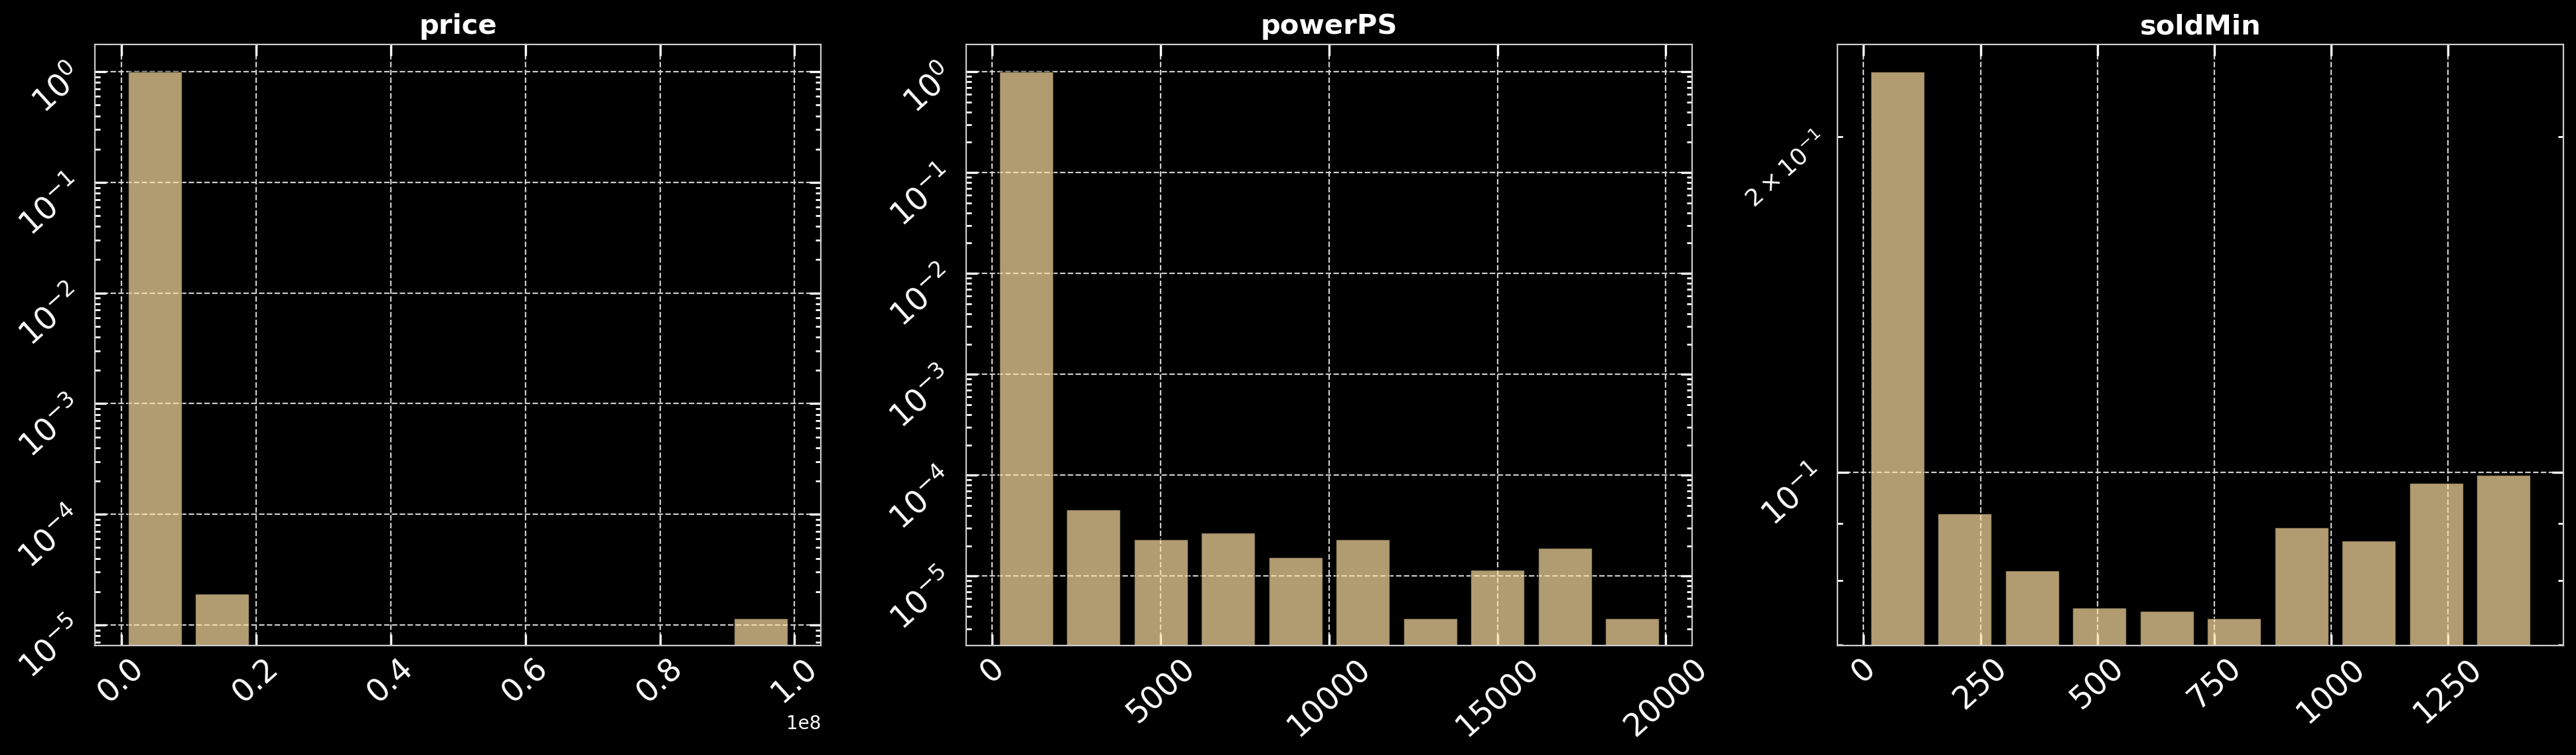
\includegraphics[width=\linewidth]{./images/fig_1_dist_pre.png}
		\captionof{figure}{The distribution of continuous features values, where some columns (here \texttt{price} and \texttt{powerPS}) are still infested with fake values.}
	\end{center}
\end{figure}

\subsubsection{Fake values in \texttt{price}}
On Fig 2. we can see, that mock values here are really huge, probably values like `999999999` or similar placeholders widely used in digital environments. They're are separates from real values on the far right side of the graph. We can easily filter these values by deleting all of them over some threshold. Let us choose this threshold to be over eg. $3$ million.

\subsubsection{Fake values in \texttt{yearOfRegistration}}
Fake values here are all over the spectrum. Feature values are ranging from \texttt{1000} to \texttt{9999}. We need to select an interval, where entries having \texttt{yearOfRegistration} values outside of this interval are dropped. The Ford T-model from 1908 is referred to be as the first "real" car usually. This means we can select a eg. 1900 as the lower limit of this interval. The upper interval should be obviously 2020.

\subsubsection{Fake values in \texttt{powerPS}}
A Bugatti Veyron's engine is approximately capped at $1200$ HP, while a main battle tank's engine can be output up to $2000$ HP on average. All values above eg. $1500$ can be dropped without hesitation.

\begin{figure}[h]
	\begin{center}
		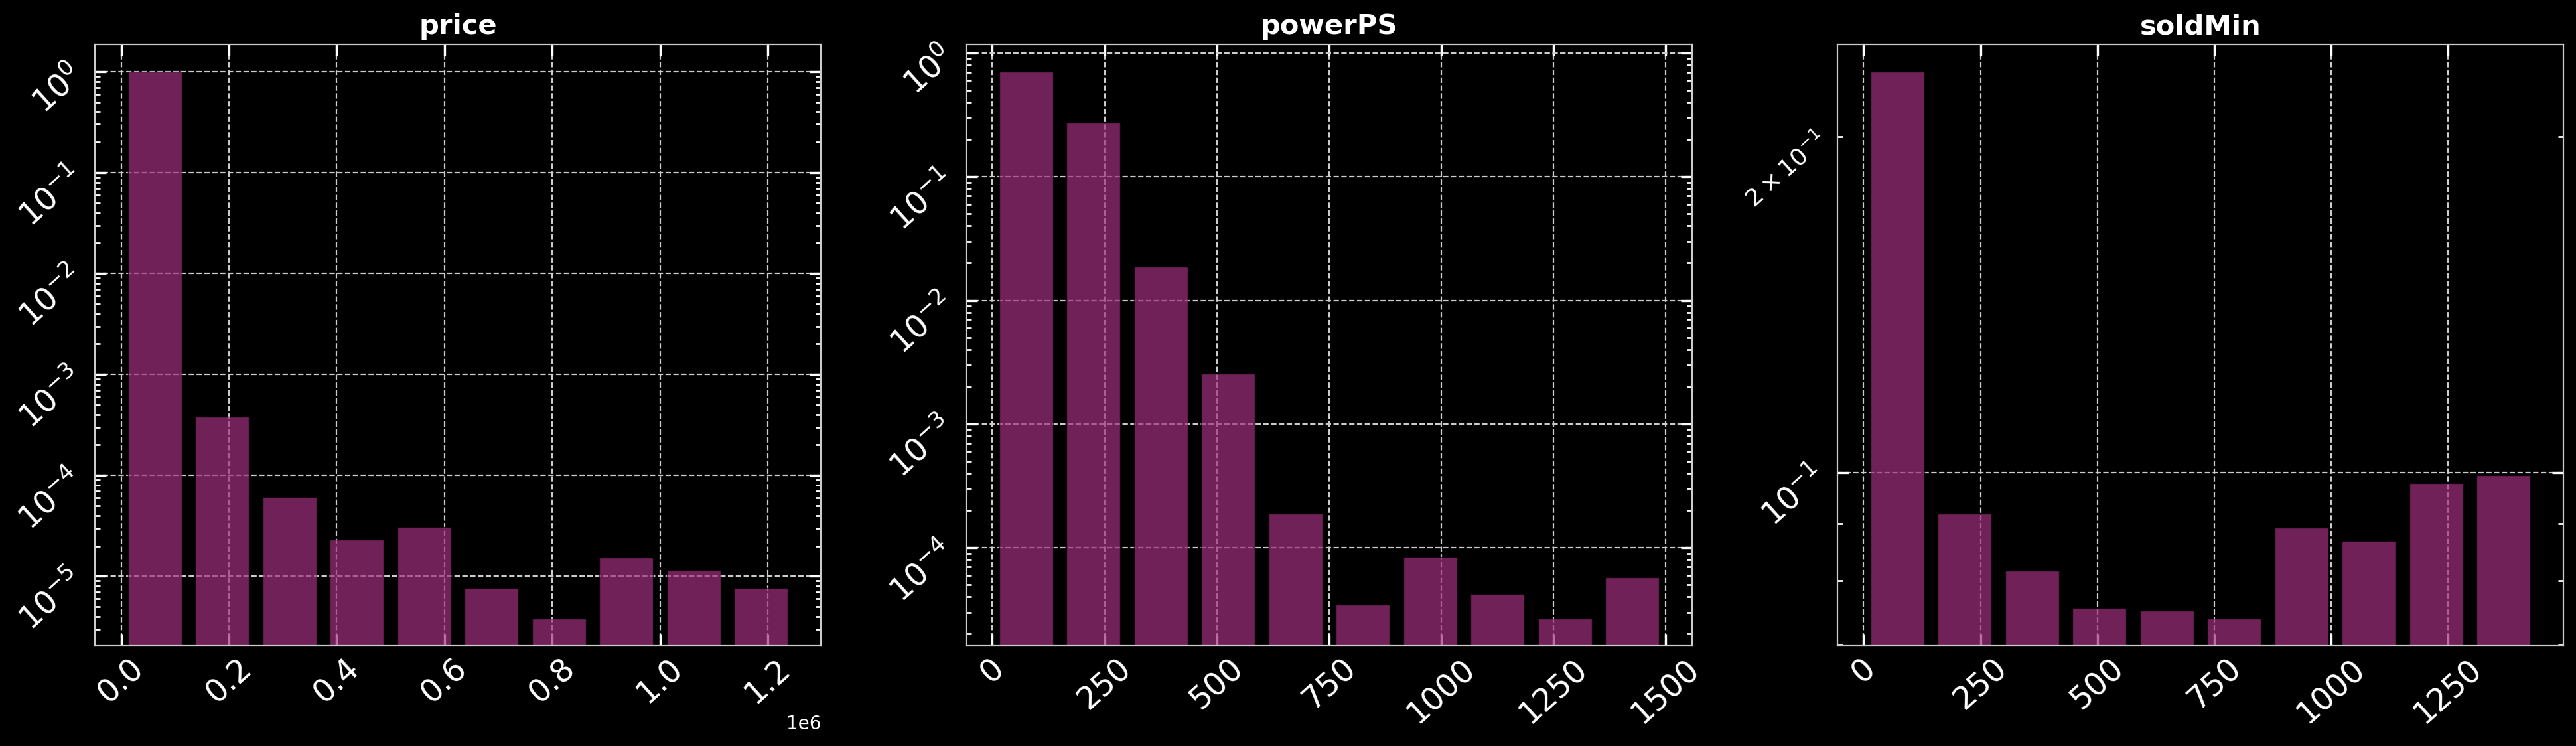
\includegraphics[width=\linewidth]{./images/fig_2_dist_after.png}
		\captionof{figure}{Distribution of continuous labels in the modified dataset after filtering out all placeholder/faulty/mock feature values. Note, that only \texttt{price} and \texttt{powerPS} were altered during the filtering here.}
	\end{center}
\end{figure}
The measures detailed above however not enough. If we look at the feature space of the continuous variables on Fig. 4. we can find other type of mock values in the dataset.

\begin{figure}[h]
	\begin{center}
		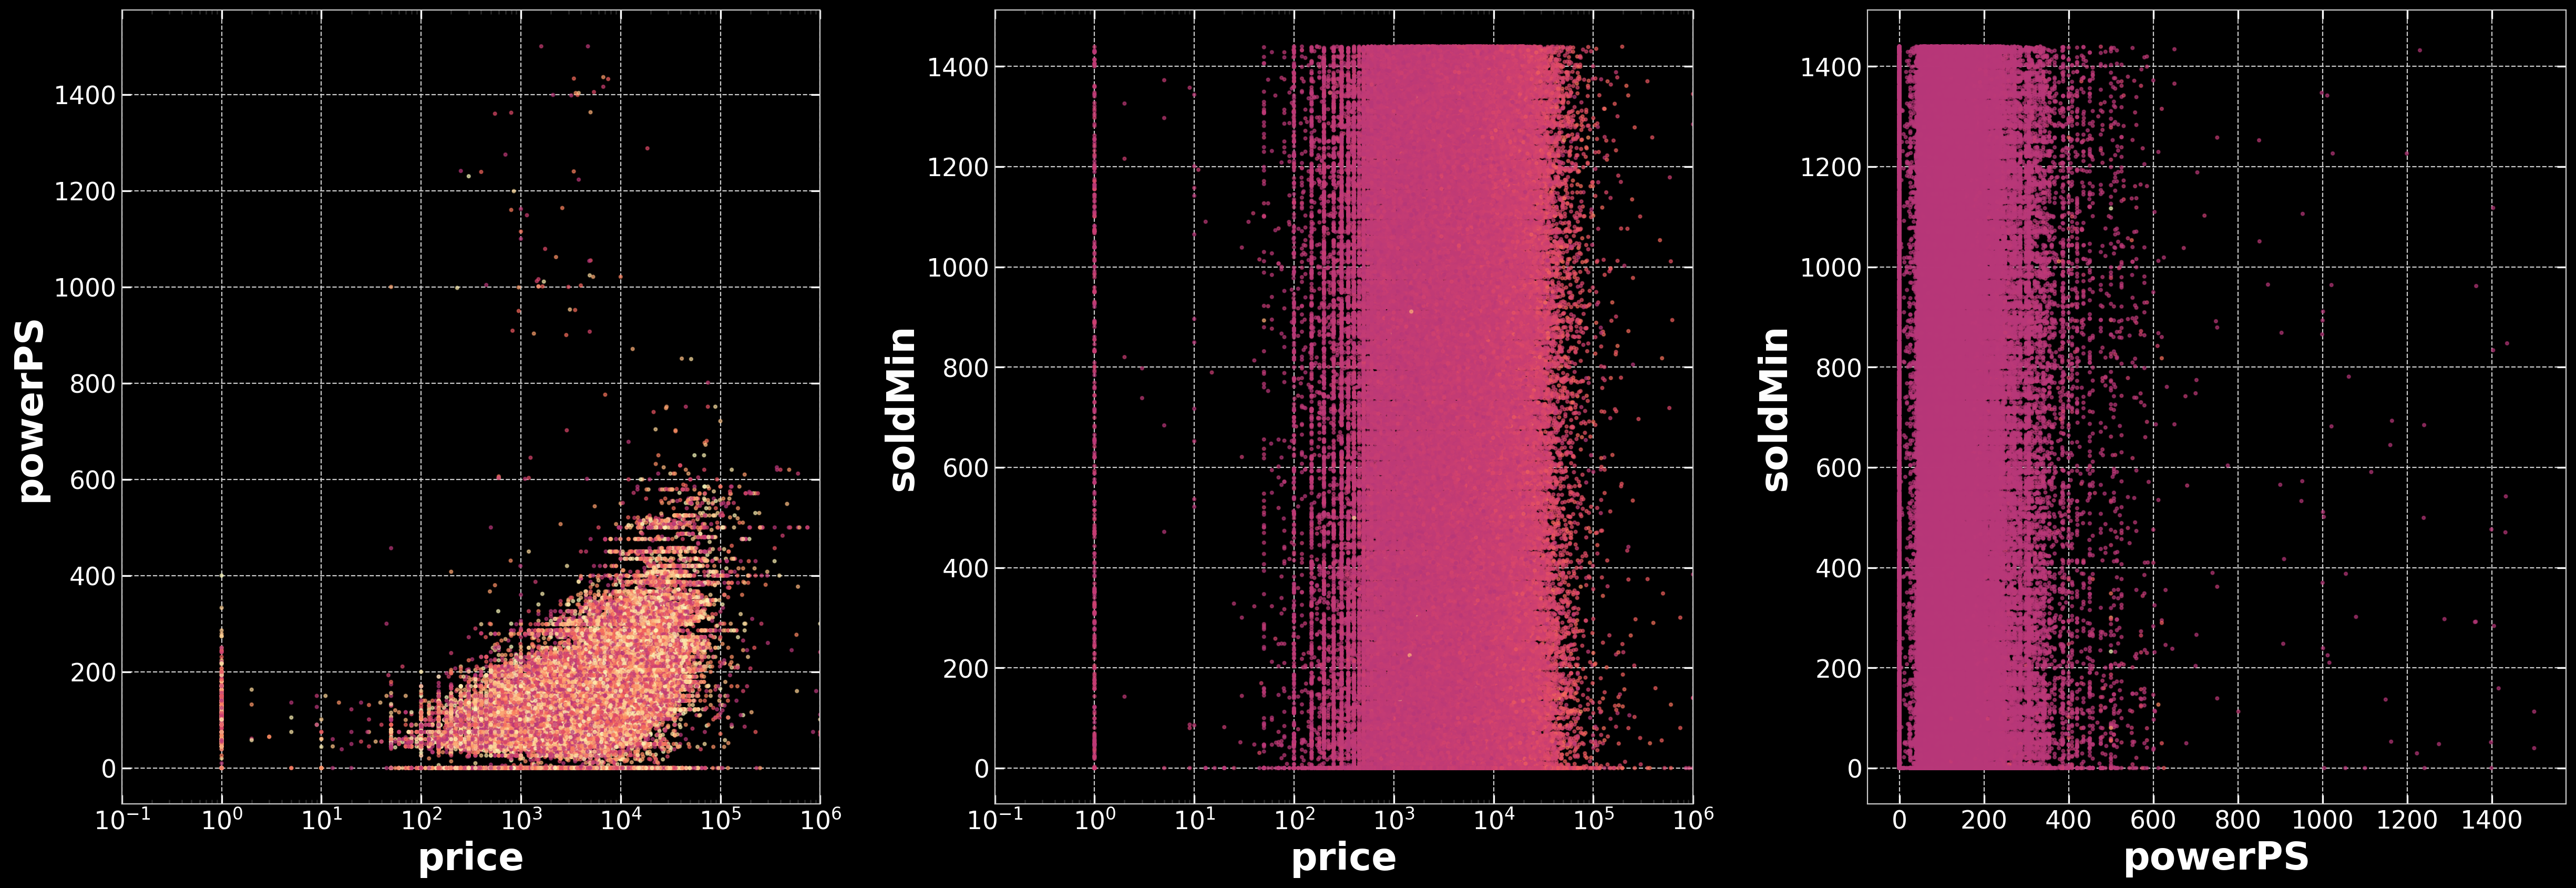
\includegraphics[width=\linewidth]{./images/fig_3_feat_space_pre.png}
		\captionof{figure}{The feature space of the remaining continuous variables. We can observe mock values in the \texttt{price} and \texttt{powerPS} features, where a lot of \texttt{price} values are given to be $1$ and a lot of \texttt{powerPS} values to be $0$.}
	\end{center}
\end{figure}
Prices - when not determined by the vendor - are usually indicated as the smallest amount of money that can be set for the advertisement in a web market. In Hungary it's eg. $1$ Ft, in the case of Ebay's panel it's probably $1$ Euro. We can see this behaviour on Fig. 4., where a lot of \texttt{price} values are simply equals to $1$.
In the case of the feature \texttt{powerPS} these mock values are equals to $0$. Obviously there are no vehicles with engine power $0$. After dropping all of these mock values, $250\,769$ number of entries remain, which should be enough to be explored using some interesting supervised learning algorithm. The features space of this final dataset can be seen on Fig. 4.

\begin{figure}[h]
	\begin{center}
		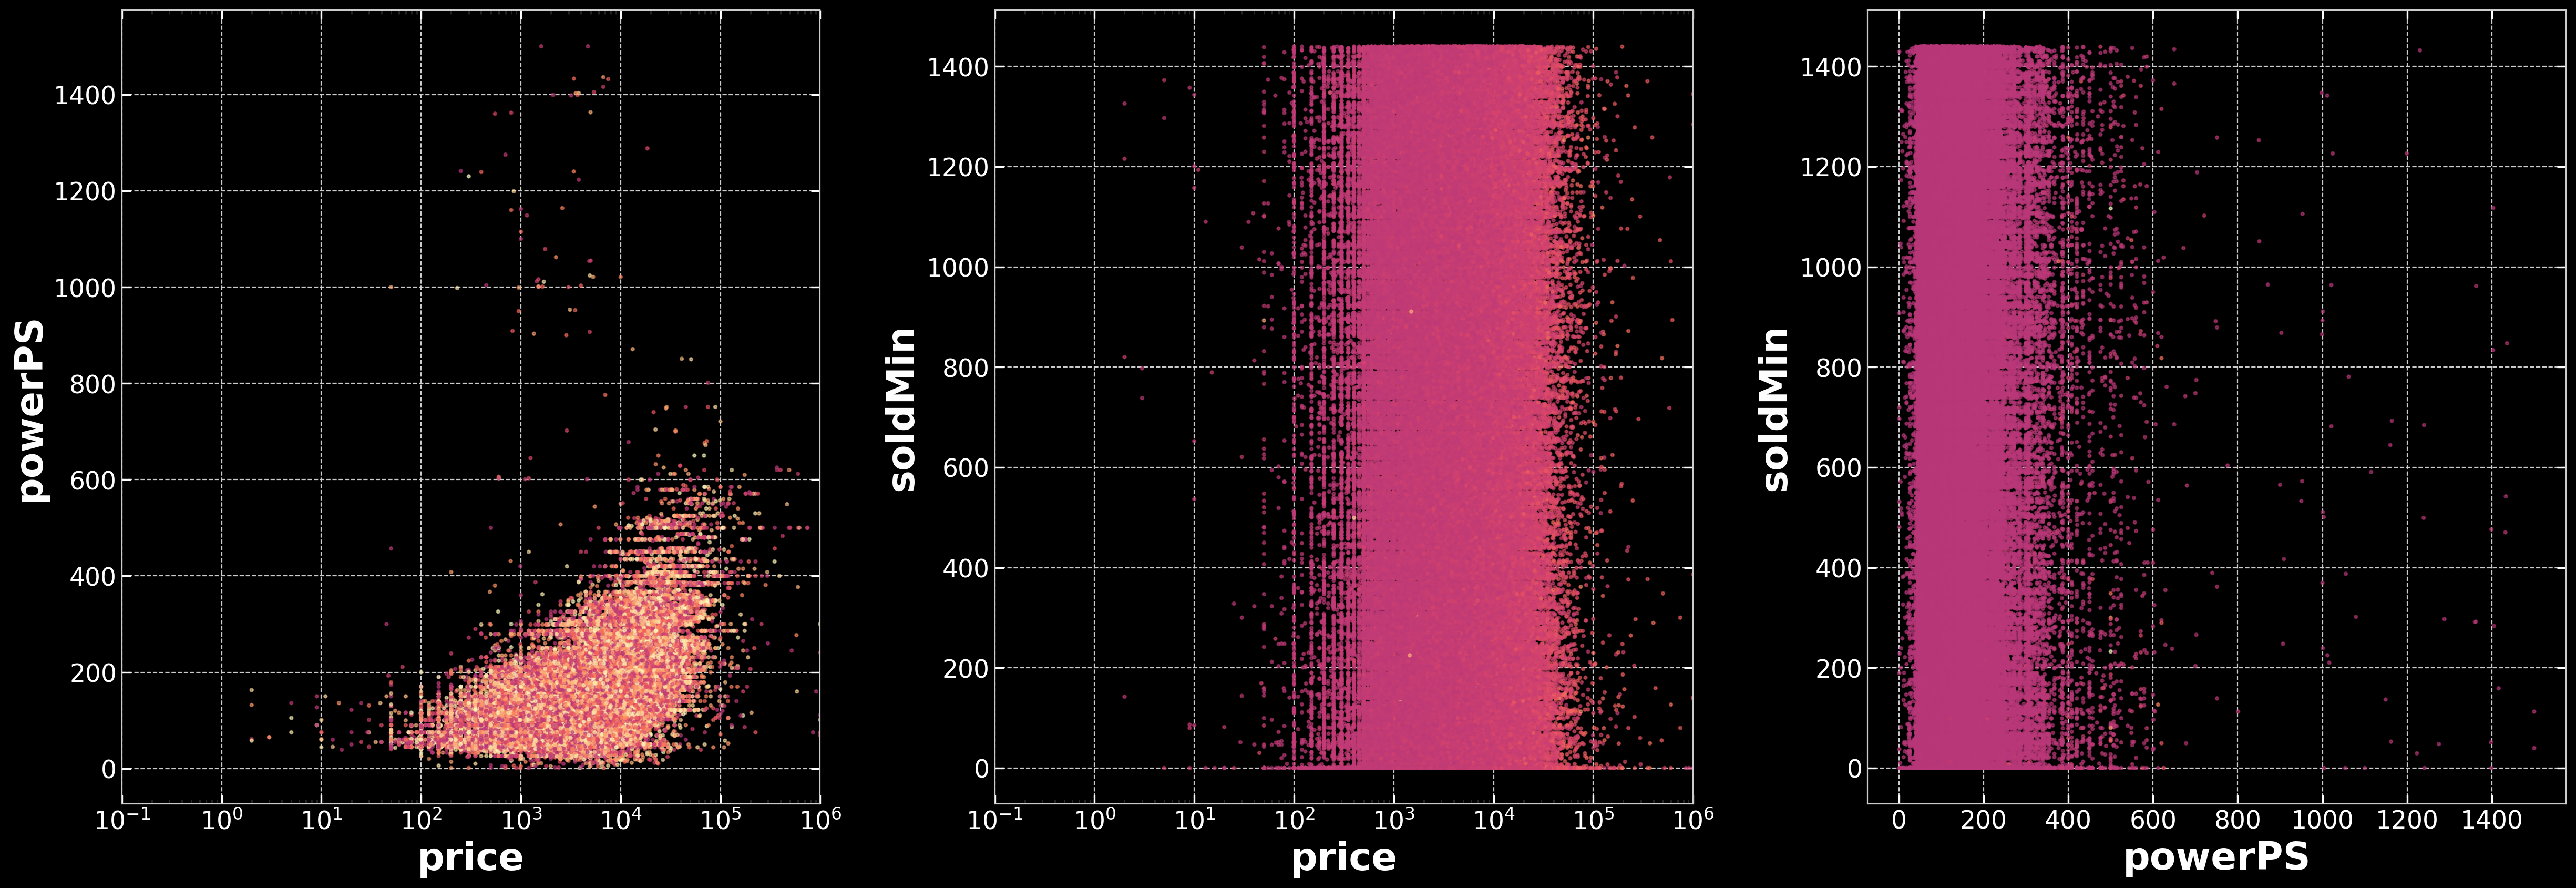
\includegraphics[width=\linewidth]{./images/fig_4_feat_space_after.png}
		\captionof{figure}{The feature space of the continuous variables after filtering out the remaining mock values too.}
	\end{center}
\end{figure}

\section{My ideas for the task}
There are a number of things can be looked into using a supervised learning algorithm. Here I'll enumerate my ideas what can explored in this used cars dataset. The main obstacle in finding a good method is arises from the structure of the dataset and the type of the remaining features. First of all, we have only $13$ features total from which only $3$ are continuous. Most other values are binary, while the feature \texttt{abtest} just a random, useless variable, which I only kept just to test it's randomness. The feature \texttt{soldMin} shows absolutely zero correlation to other continuous variables as seen of Fig. 3. and Fig. 4., and it behaves just like white or pink noise.

\subsection{Predicting binary labels from continuous features}
My first ideas was to explore, whether can I predict the binary labels (\texttt{gearbox} and \texttt{notRepairedDamage}) from the continuous features (\texttt{price}, \texttt{powerPS} and \texttt{soldMin})? Basically I at the beginning I had no idea what type of connection is there between them, so I tried various linear models in this case. Namely linear and logistic regression and a ridge classifier model. I've splitted the dataset into a training and test part with a proportion of 4:1 respectively. I've trained all models on the same train dataset and made predictions for the same test set. My results can be seen on Fig. 5, Fig. 6. and Fig. 7.

% LINEAR REGRESSION
\begin{figure}[h]
	\begin{center}
		\begin{subfigure}{0.32\textwidth}
			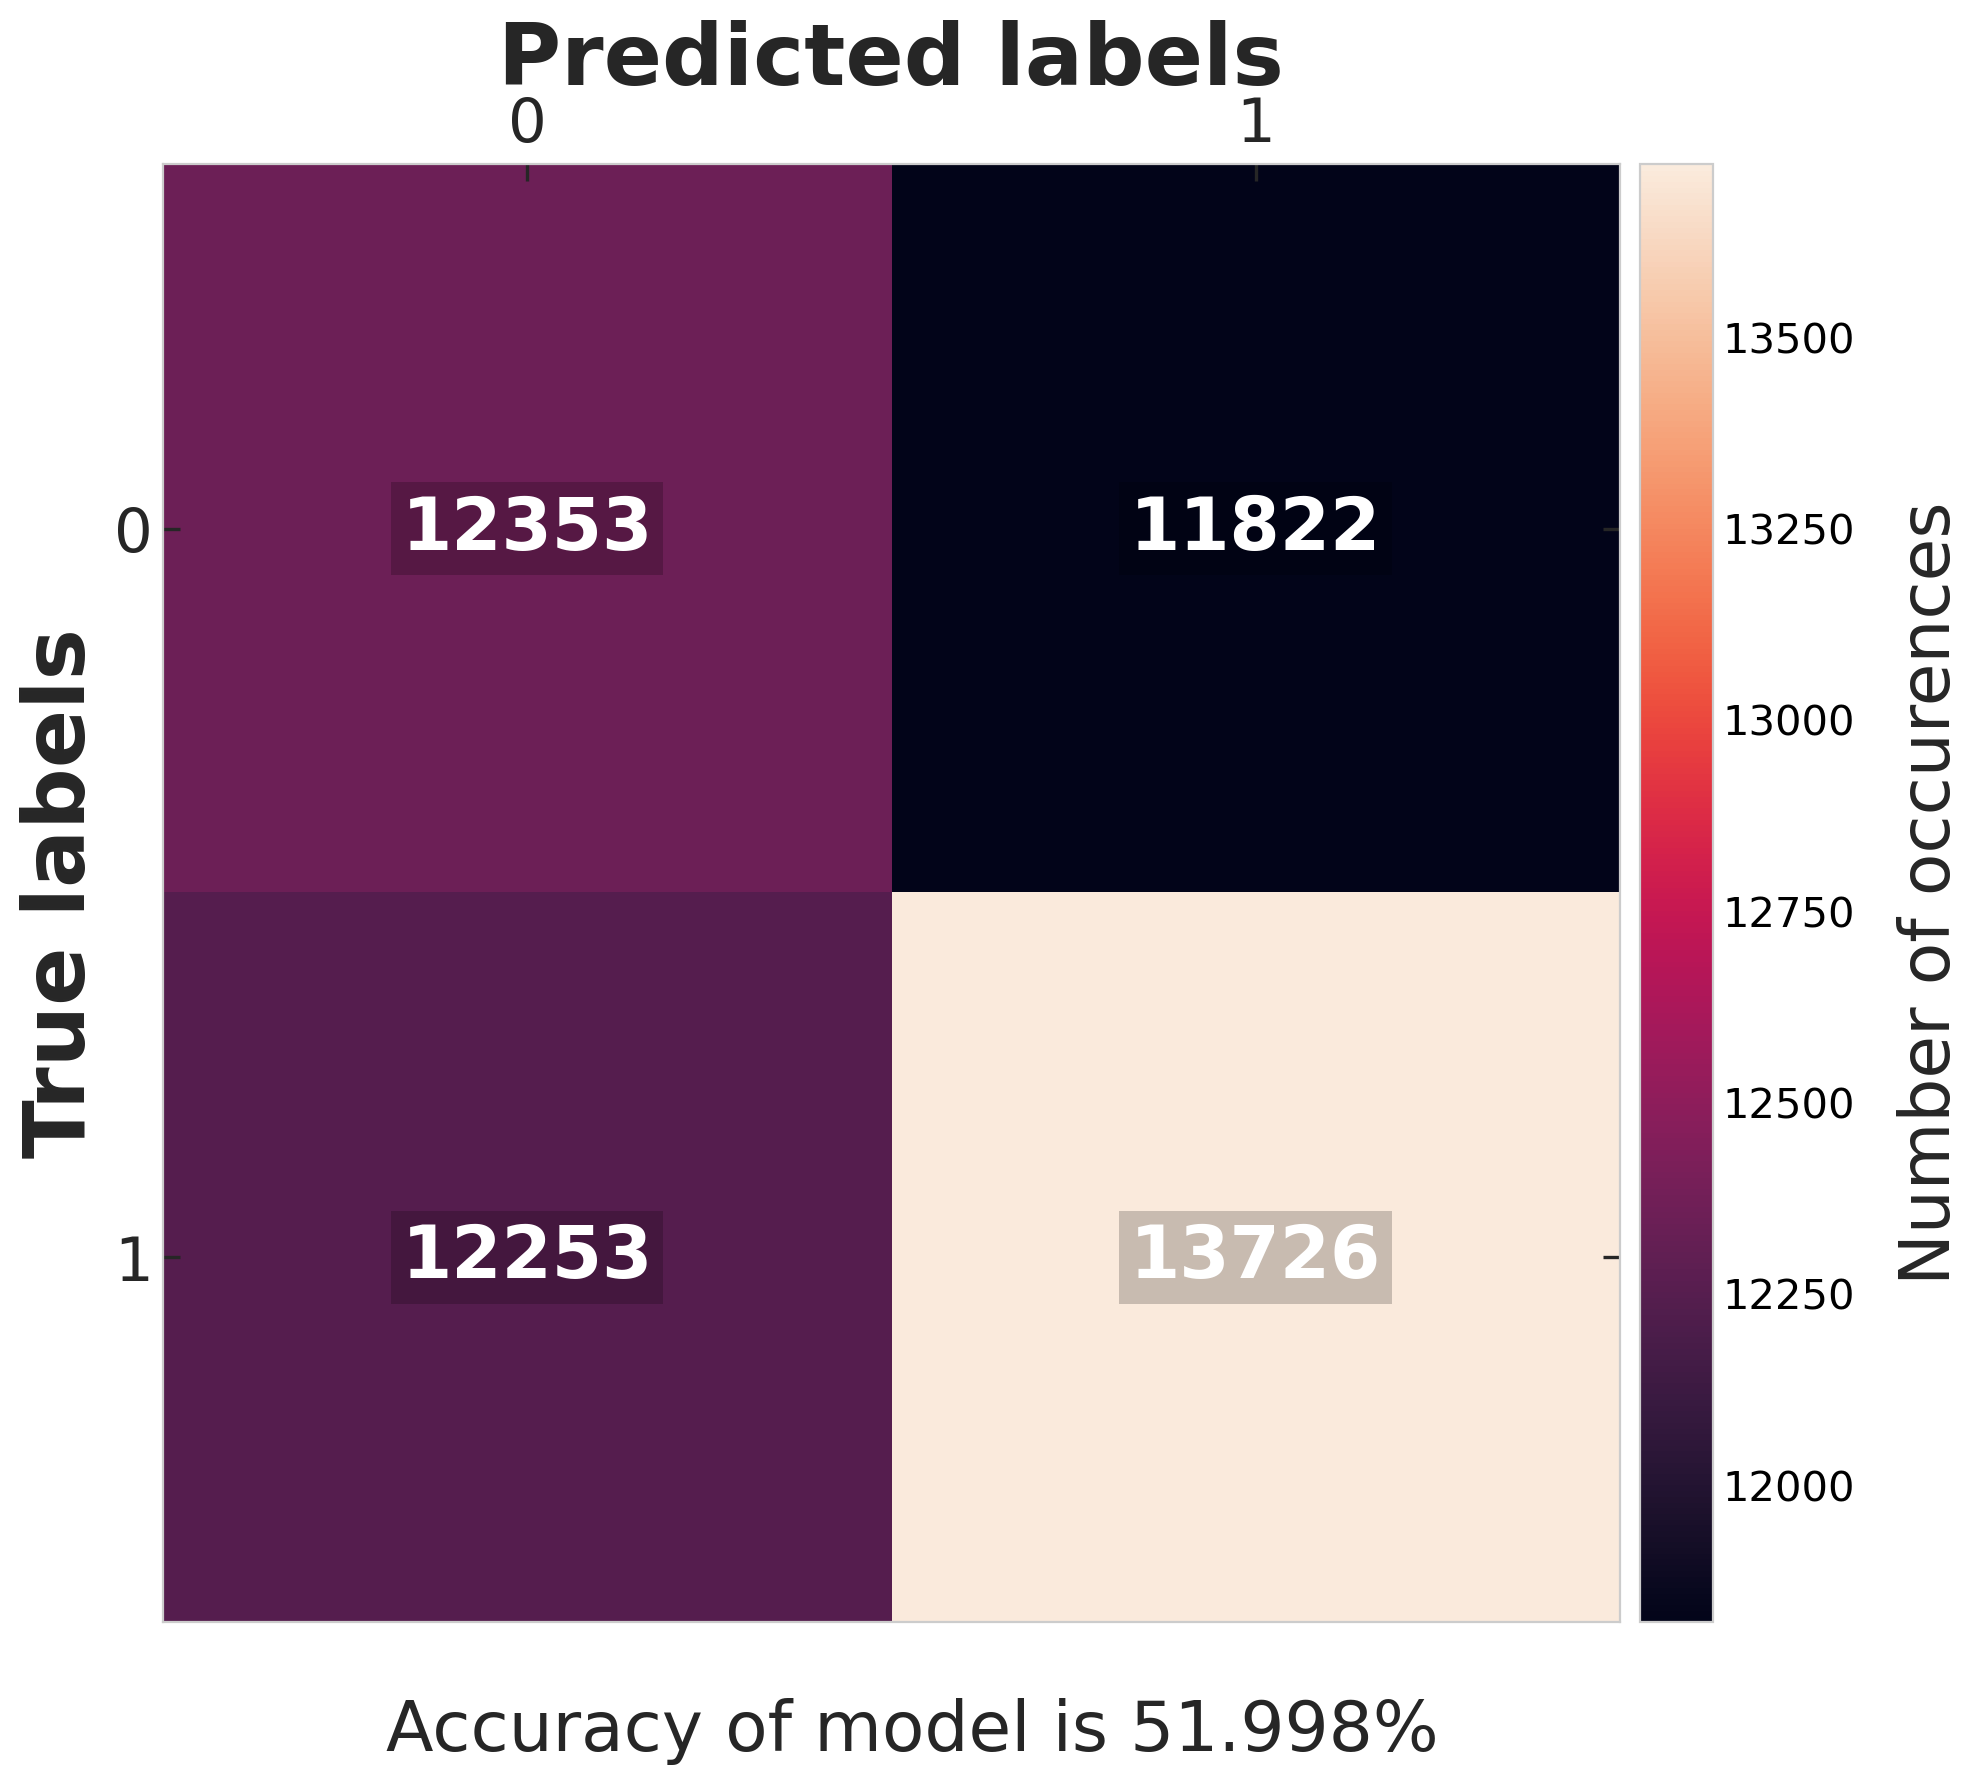
\includegraphics[width=0.99\linewidth]{./images/fig_6_linear_abtest.png} 
			\caption{Predicting \texttt{abtest}}
		\end{subfigure}
		\begin{subfigure}{0.32\textwidth}
			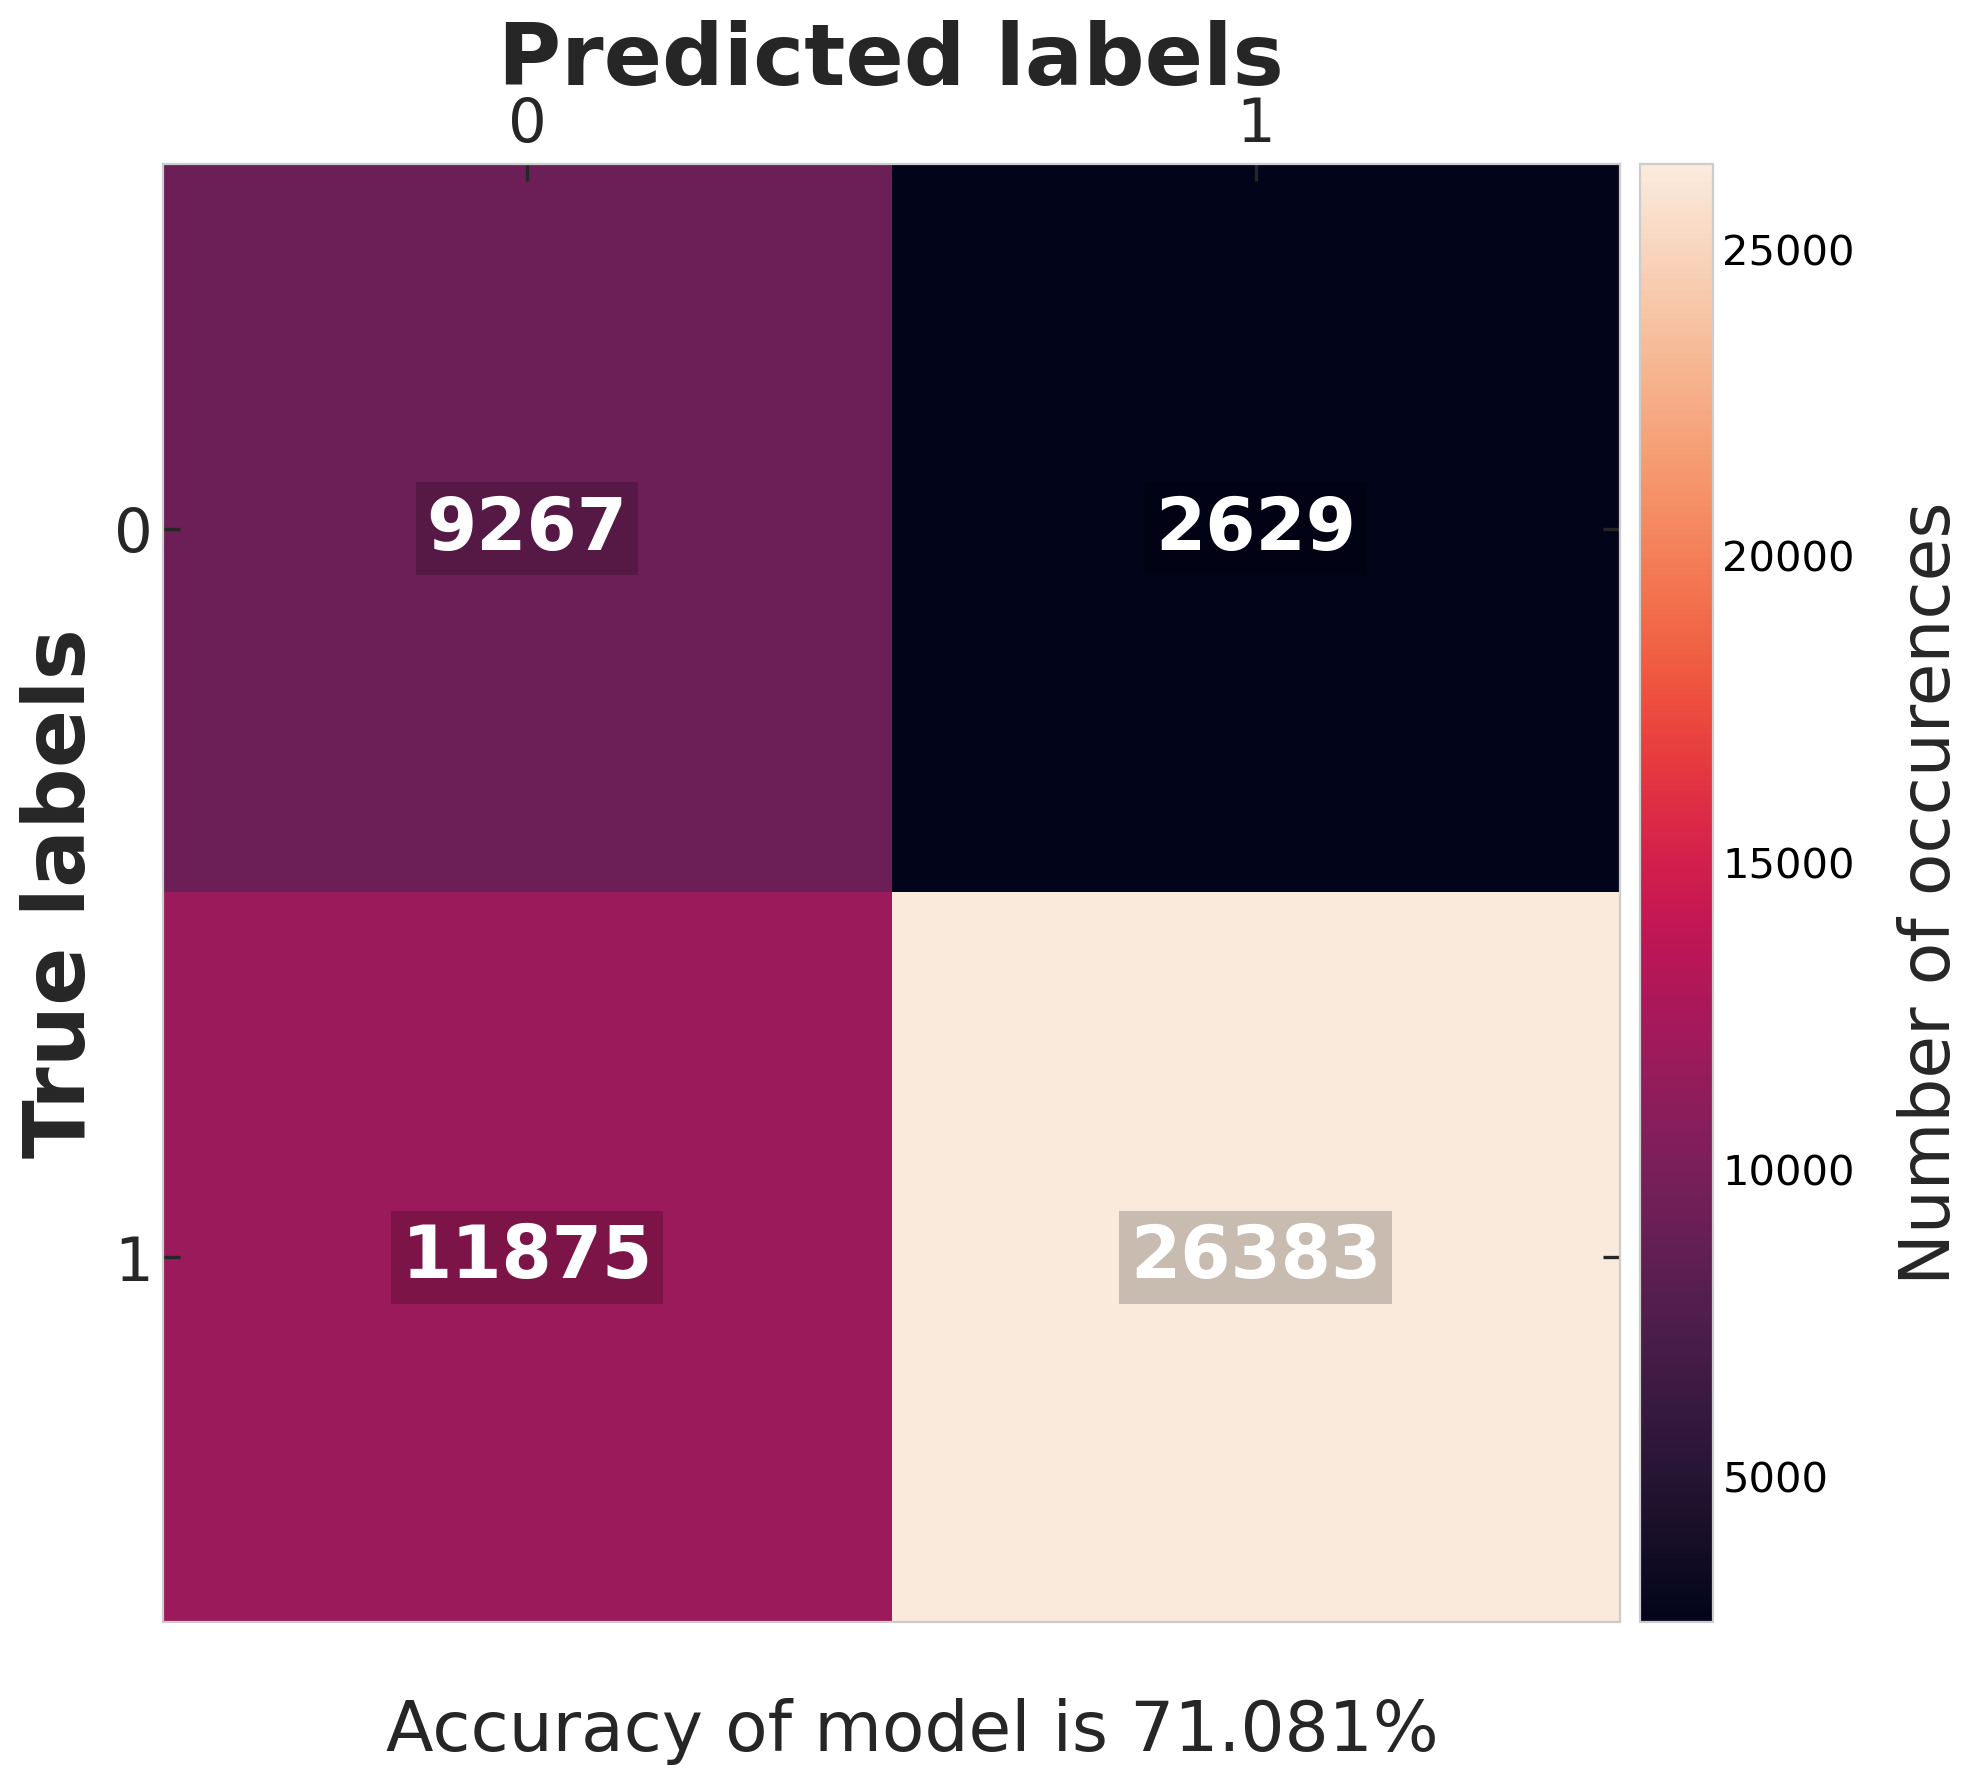
\includegraphics[width=0.99\linewidth]{./images/fig_7_linear_gearbox.png} 
			\caption{Predicting \texttt{gearbox}}
		\end{subfigure}
		\begin{subfigure}{0.32\textwidth}
			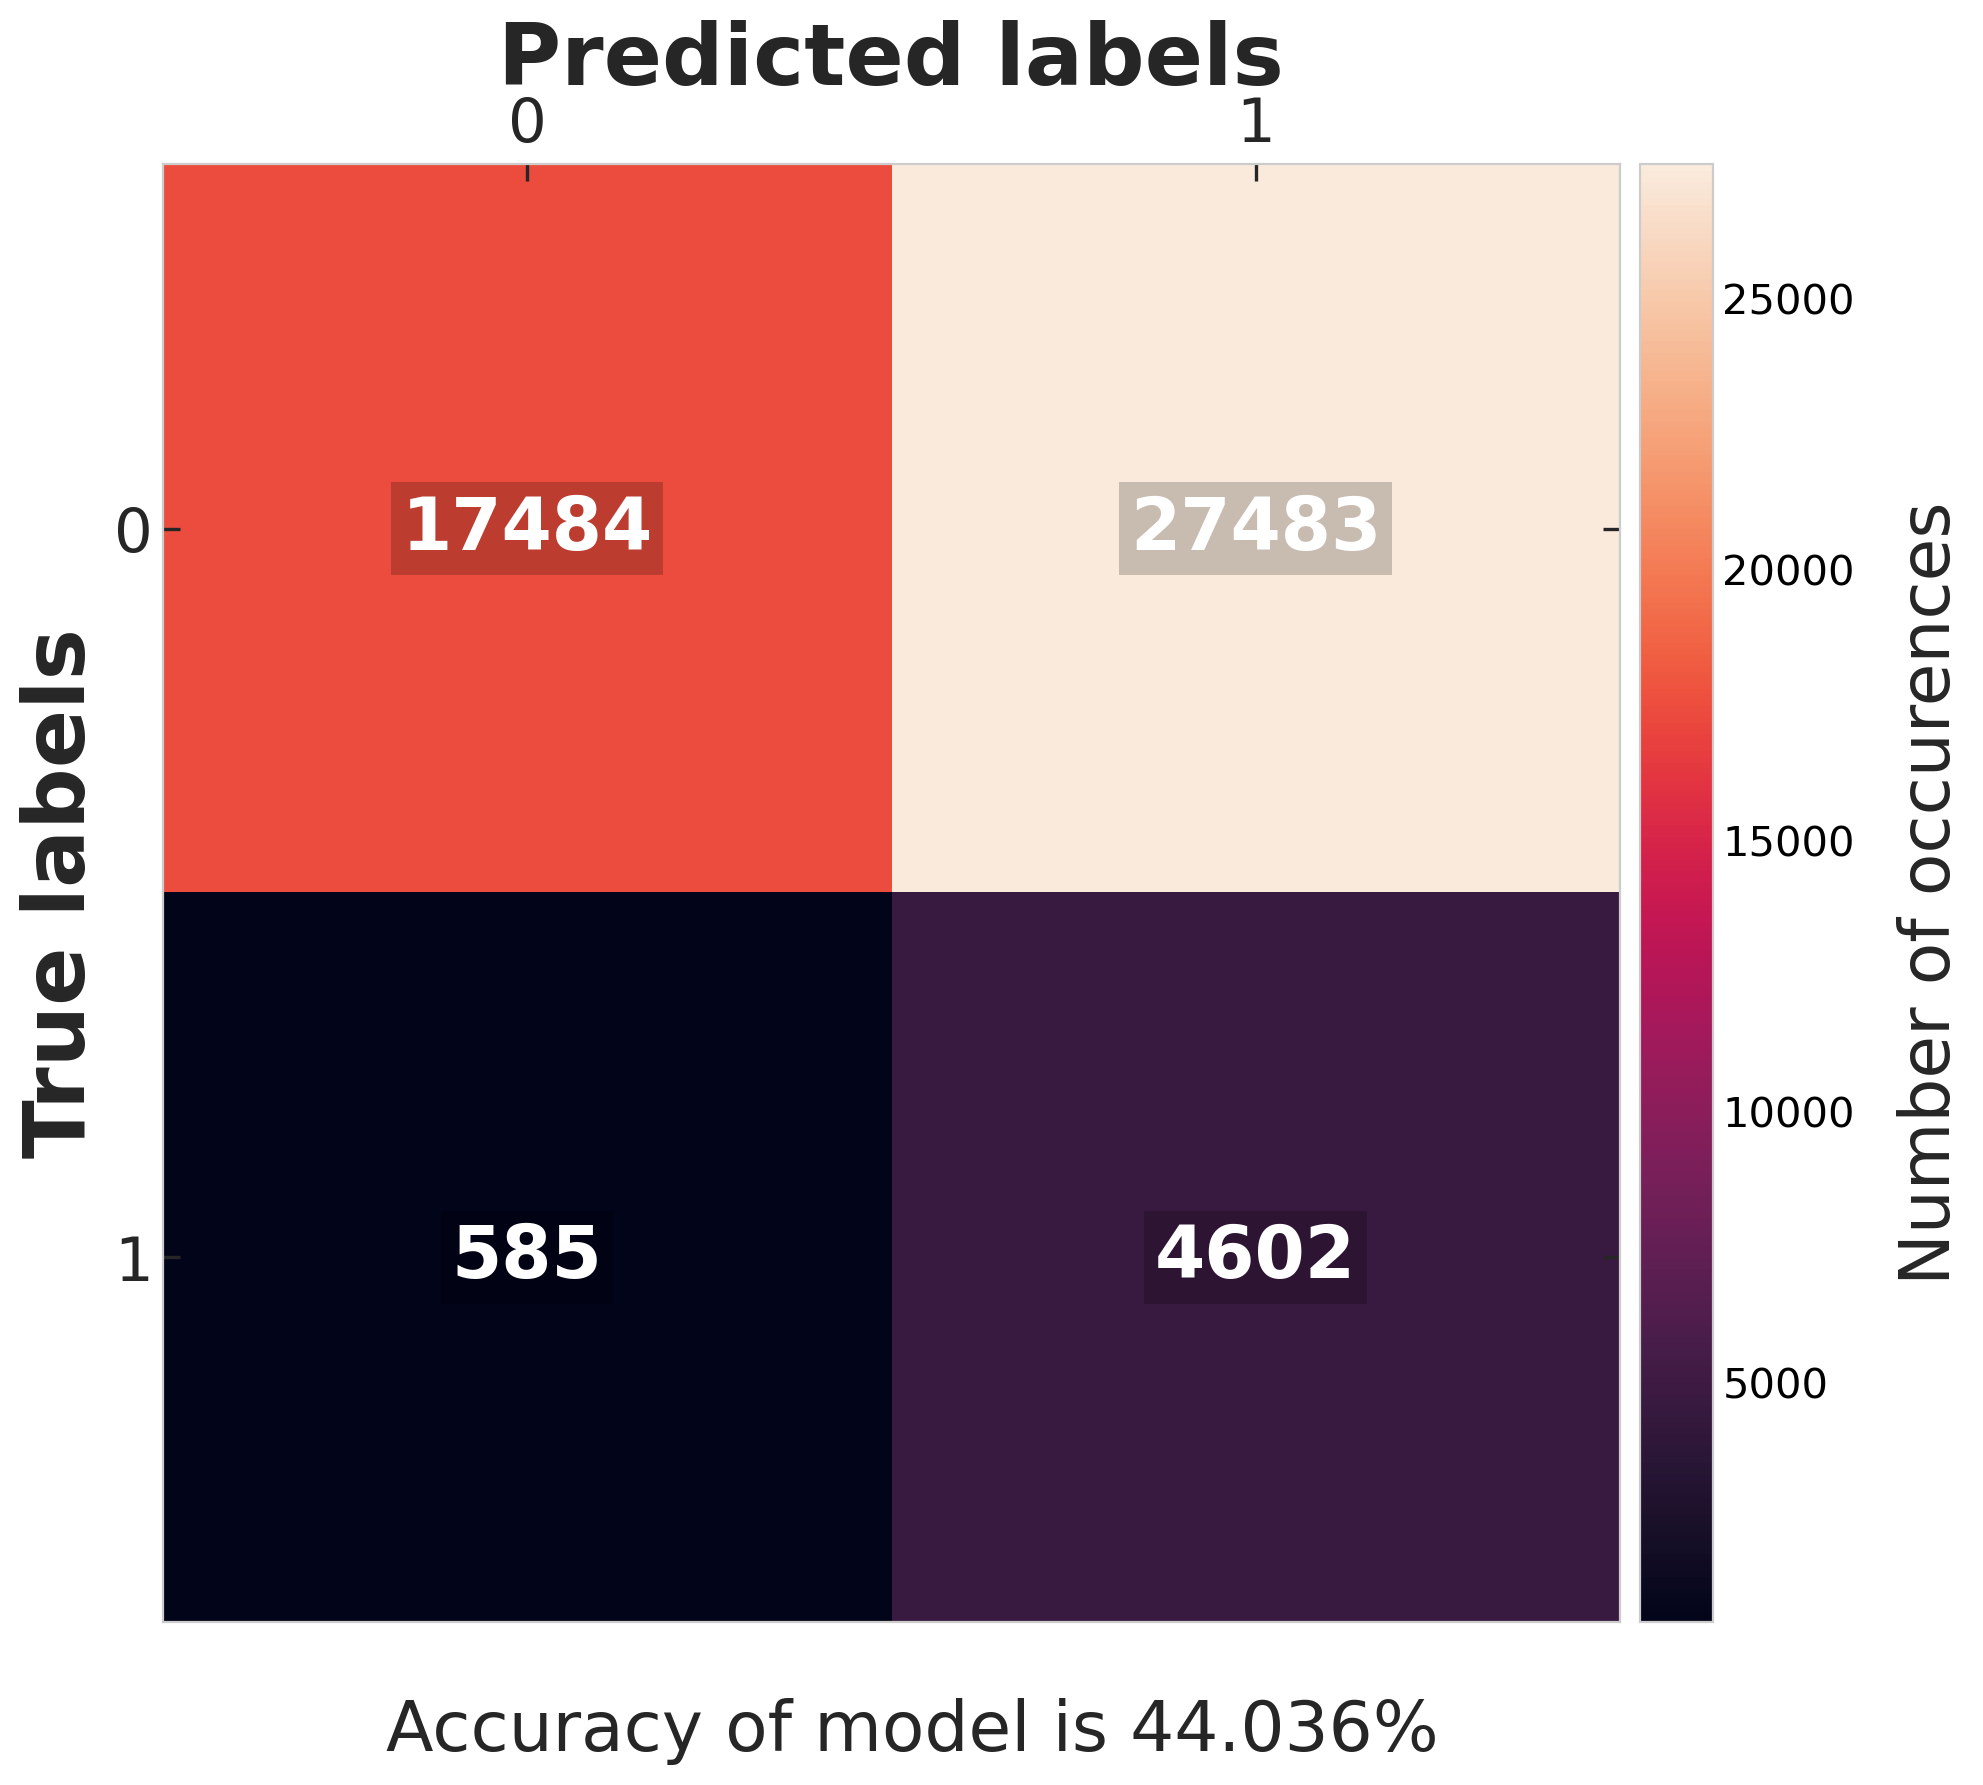
\includegraphics[width=0.99\linewidth]{./images/fig_8_linear_notrepaired.png} 
			\caption{Predicting \texttt{notRepairedDamage}}
		\end{subfigure}
		\captionof{figure}{Training a simple linear regression on the continuous variables to predict binary labels in the dataset. As it was projected, \texttt{abtest} values are indeed totally random, the simple linear regression returns with $\approx 50\%$ of accuracy. \texttt{notRepairedDamage} seems also random, because of the low model accuracy. The prediction of the \texttt{gearbox} variable however seems okay.}
	\end{center}
\end{figure}

% LOGISTIC REGRESSION
\begin{figure}[h]
	\begin{center}
		\begin{subfigure}{0.32\textwidth}
			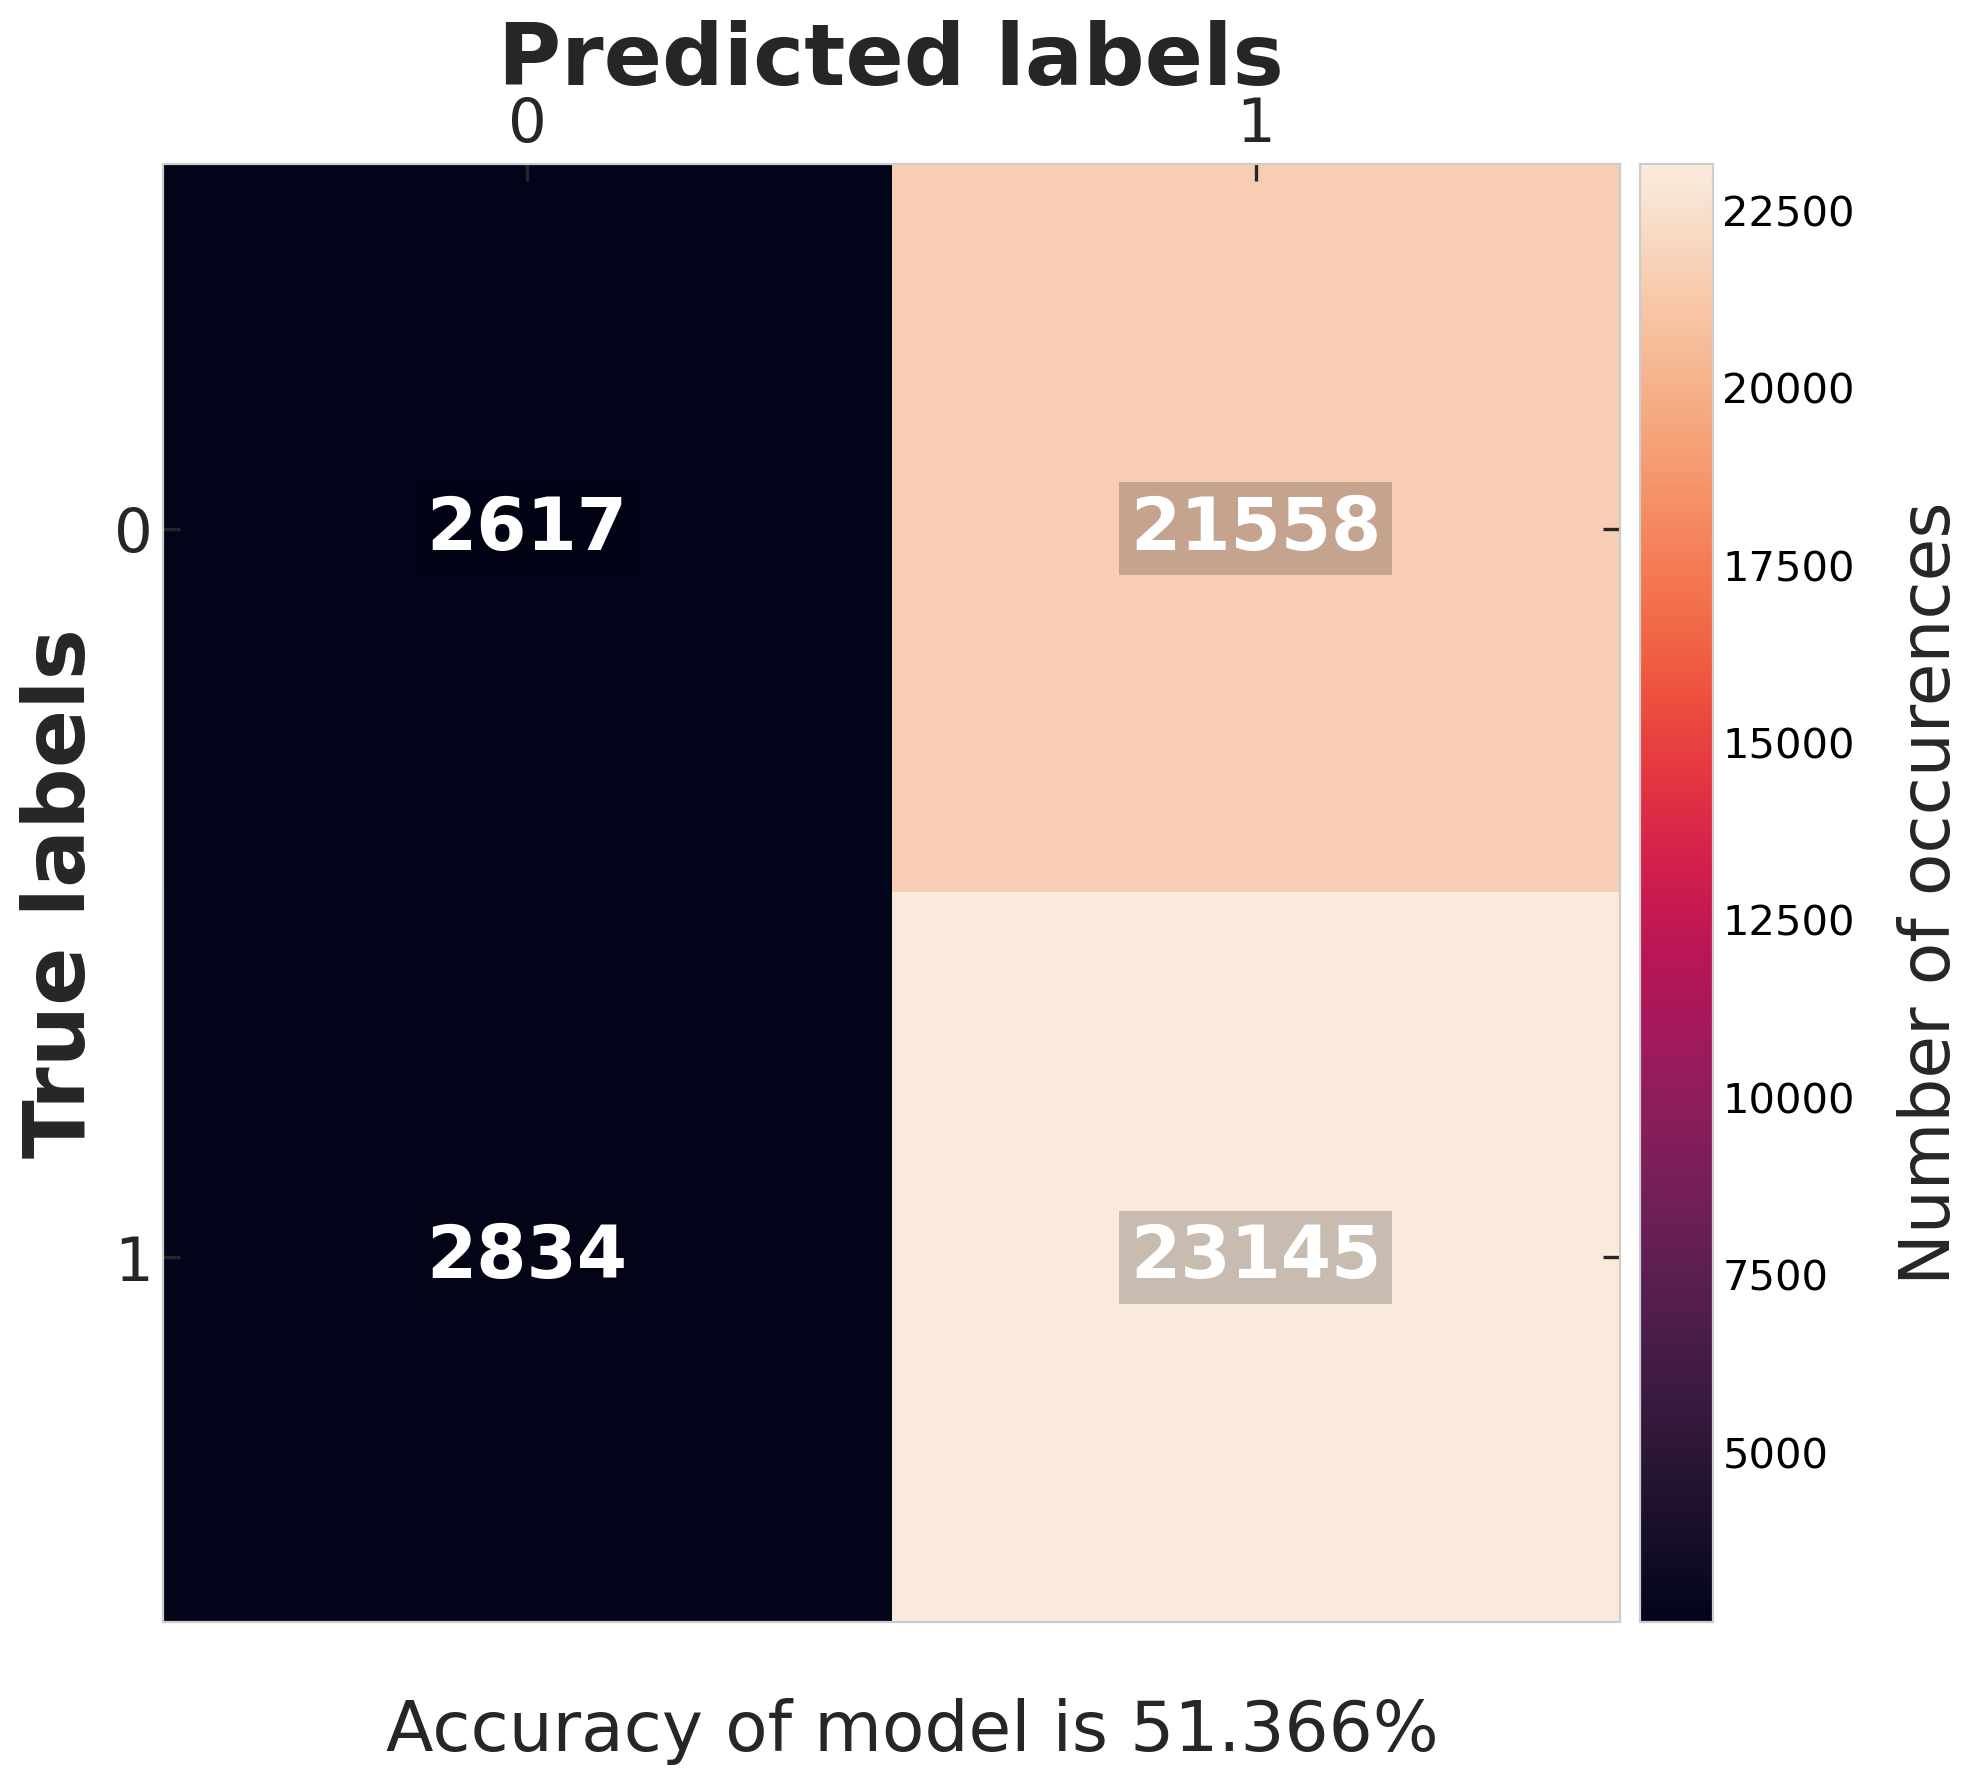
\includegraphics[width=0.99\linewidth]{./images/fig_9_logistic_abtest.png} 
			\caption{Predicting \texttt{abtest}}
		\end{subfigure}
		\begin{subfigure}{0.32\textwidth}
			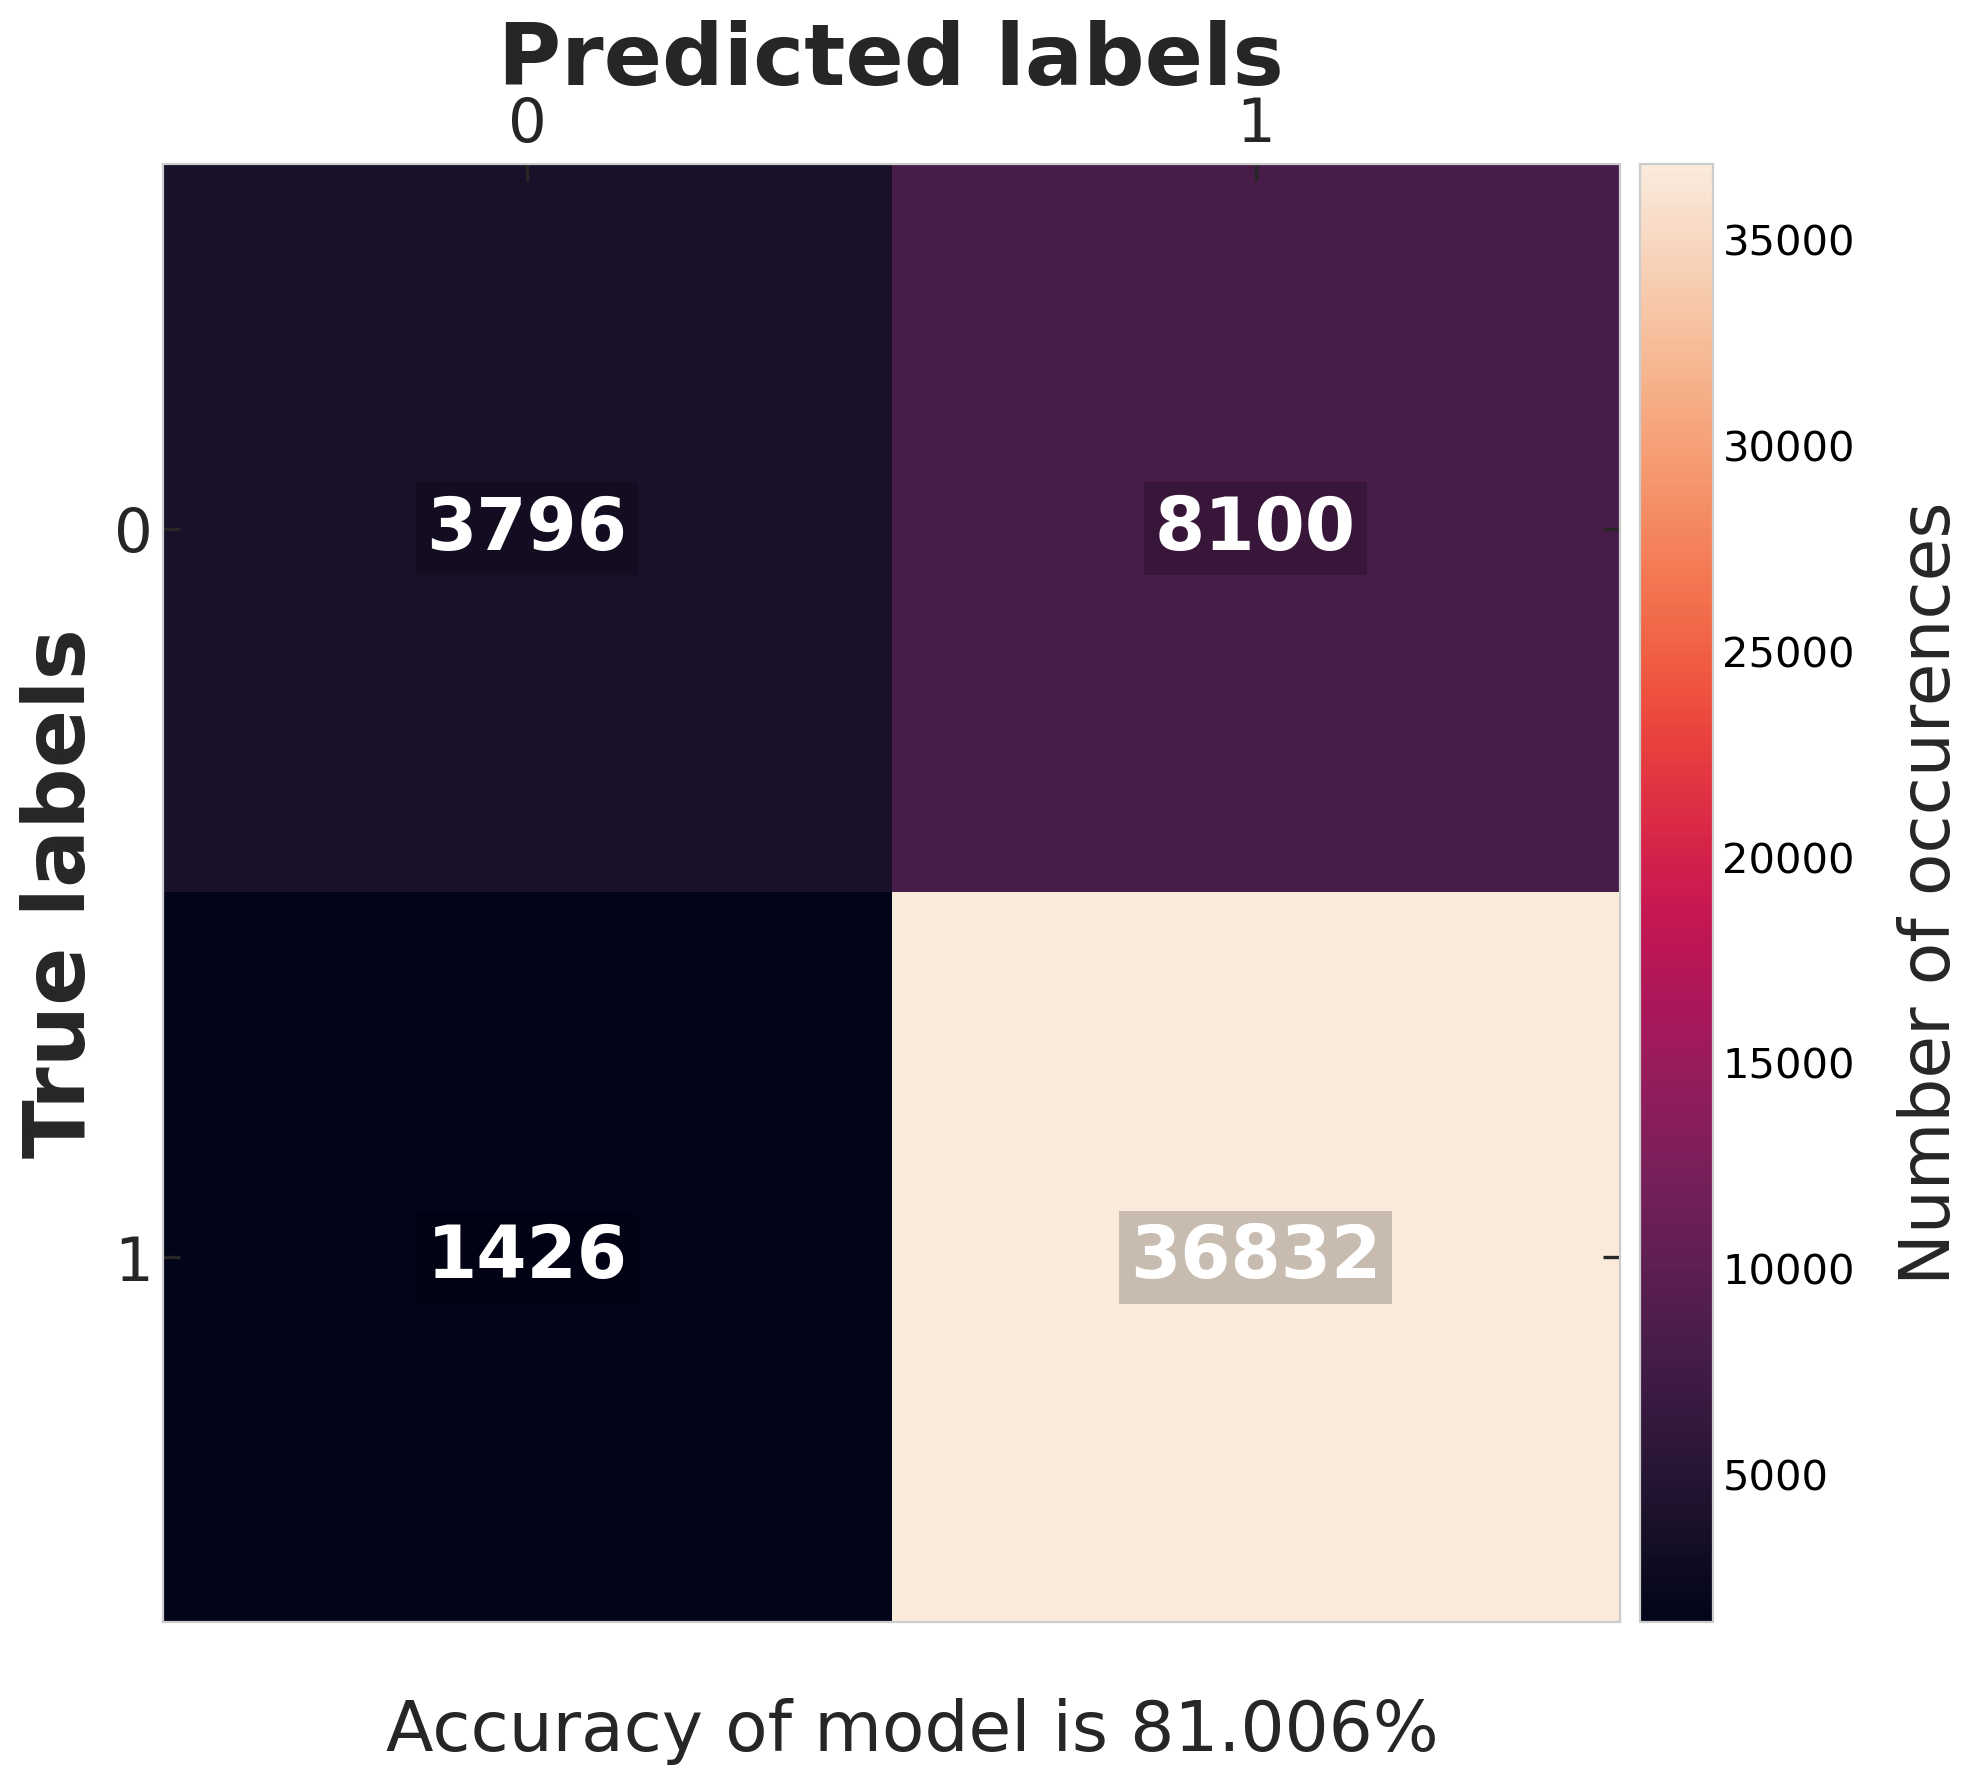
\includegraphics[width=0.99\linewidth]{./images/fig_10_logistic_gearbox.png} 
			\caption{Predicting \texttt{gearbox}}
		\end{subfigure}
		\begin{subfigure}{0.32\textwidth}
			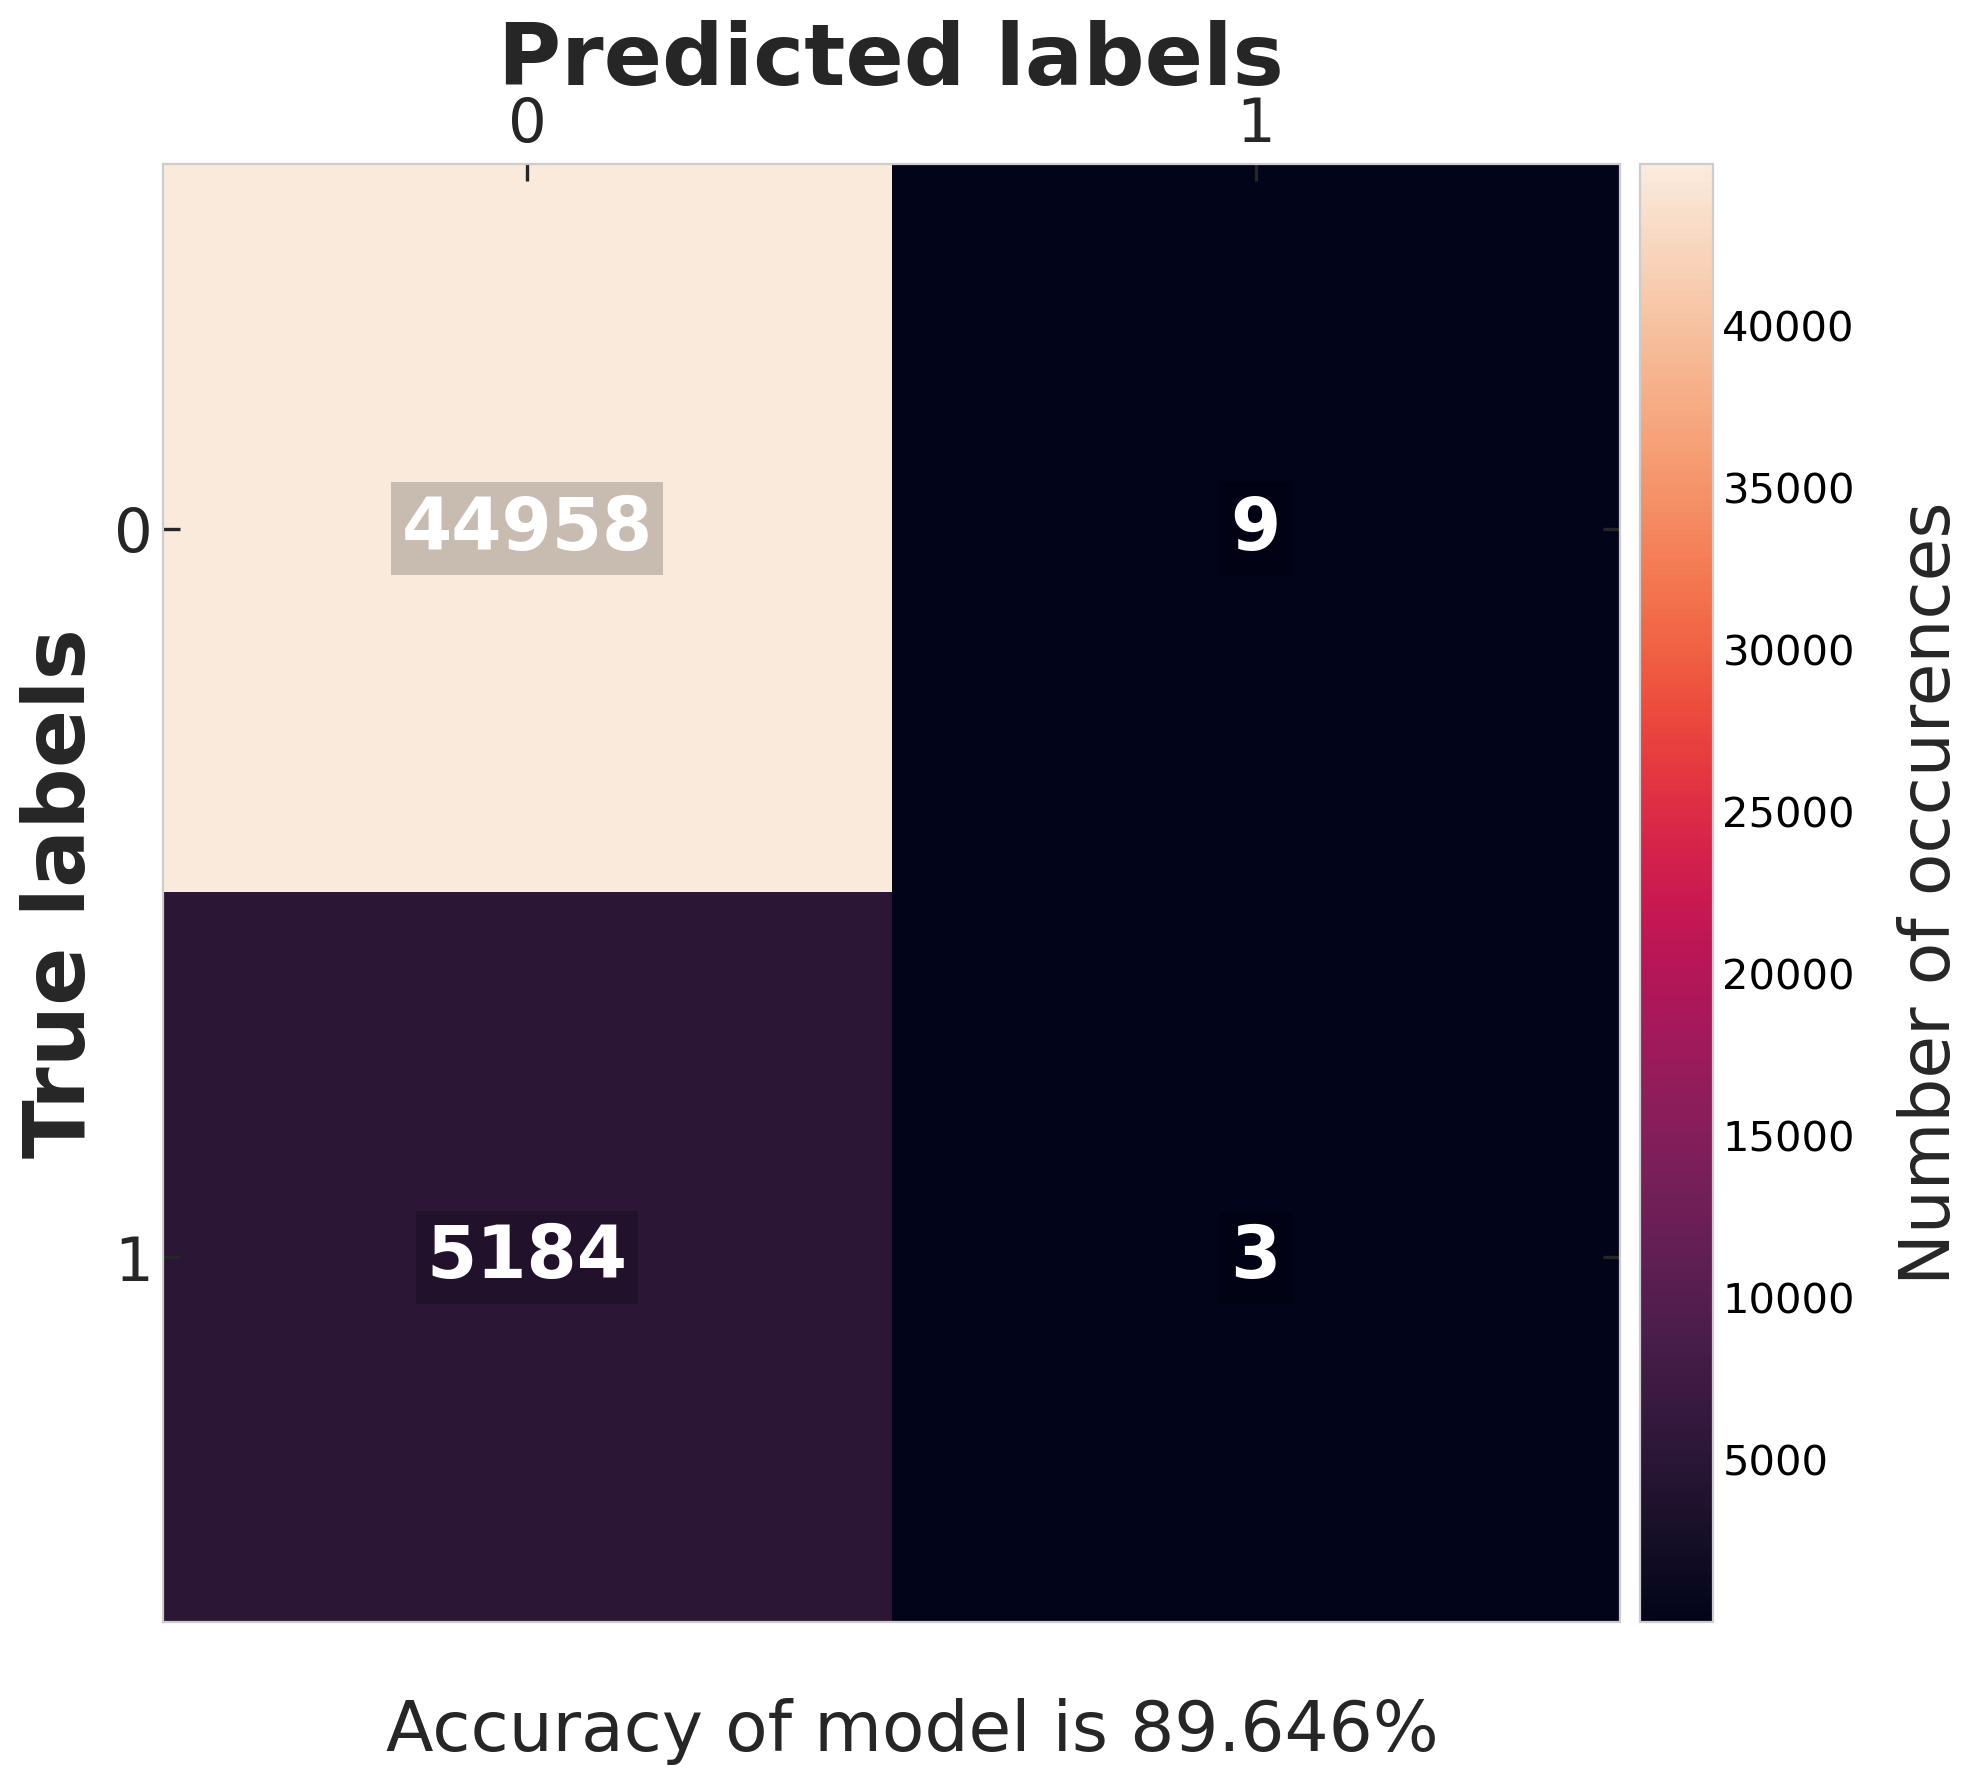
\includegraphics[width=0.99\linewidth]{./images/fig_11_logistic_notrepaired.png} 
			\caption{Predicting \texttt{notRepairedDamage}}
		\end{subfigure}
		\captionof{figure}{Training a simple logistic regression on the continuous variables to predict binary labels in the dataset. Accuracy for \texttt{abtest} is again $\approx 50\%$, while the prediction of \texttt{gearbox} is even higher than before. However it seems so that the model is heavily biased, and the \texttt{gearbox} accuracy is good just because the prediction was the same for most of the entries in the dataset. This behaviour can be observed in the case of \texttt{notRepairedDamage}, where the high accuracy is obviously due to overfitting.}
	\end{center}
\end{figure}

% RIDGE CLASSIFIER
\begin{figure}[h]
	\begin{center}
		\begin{subfigure}{0.32\textwidth}
			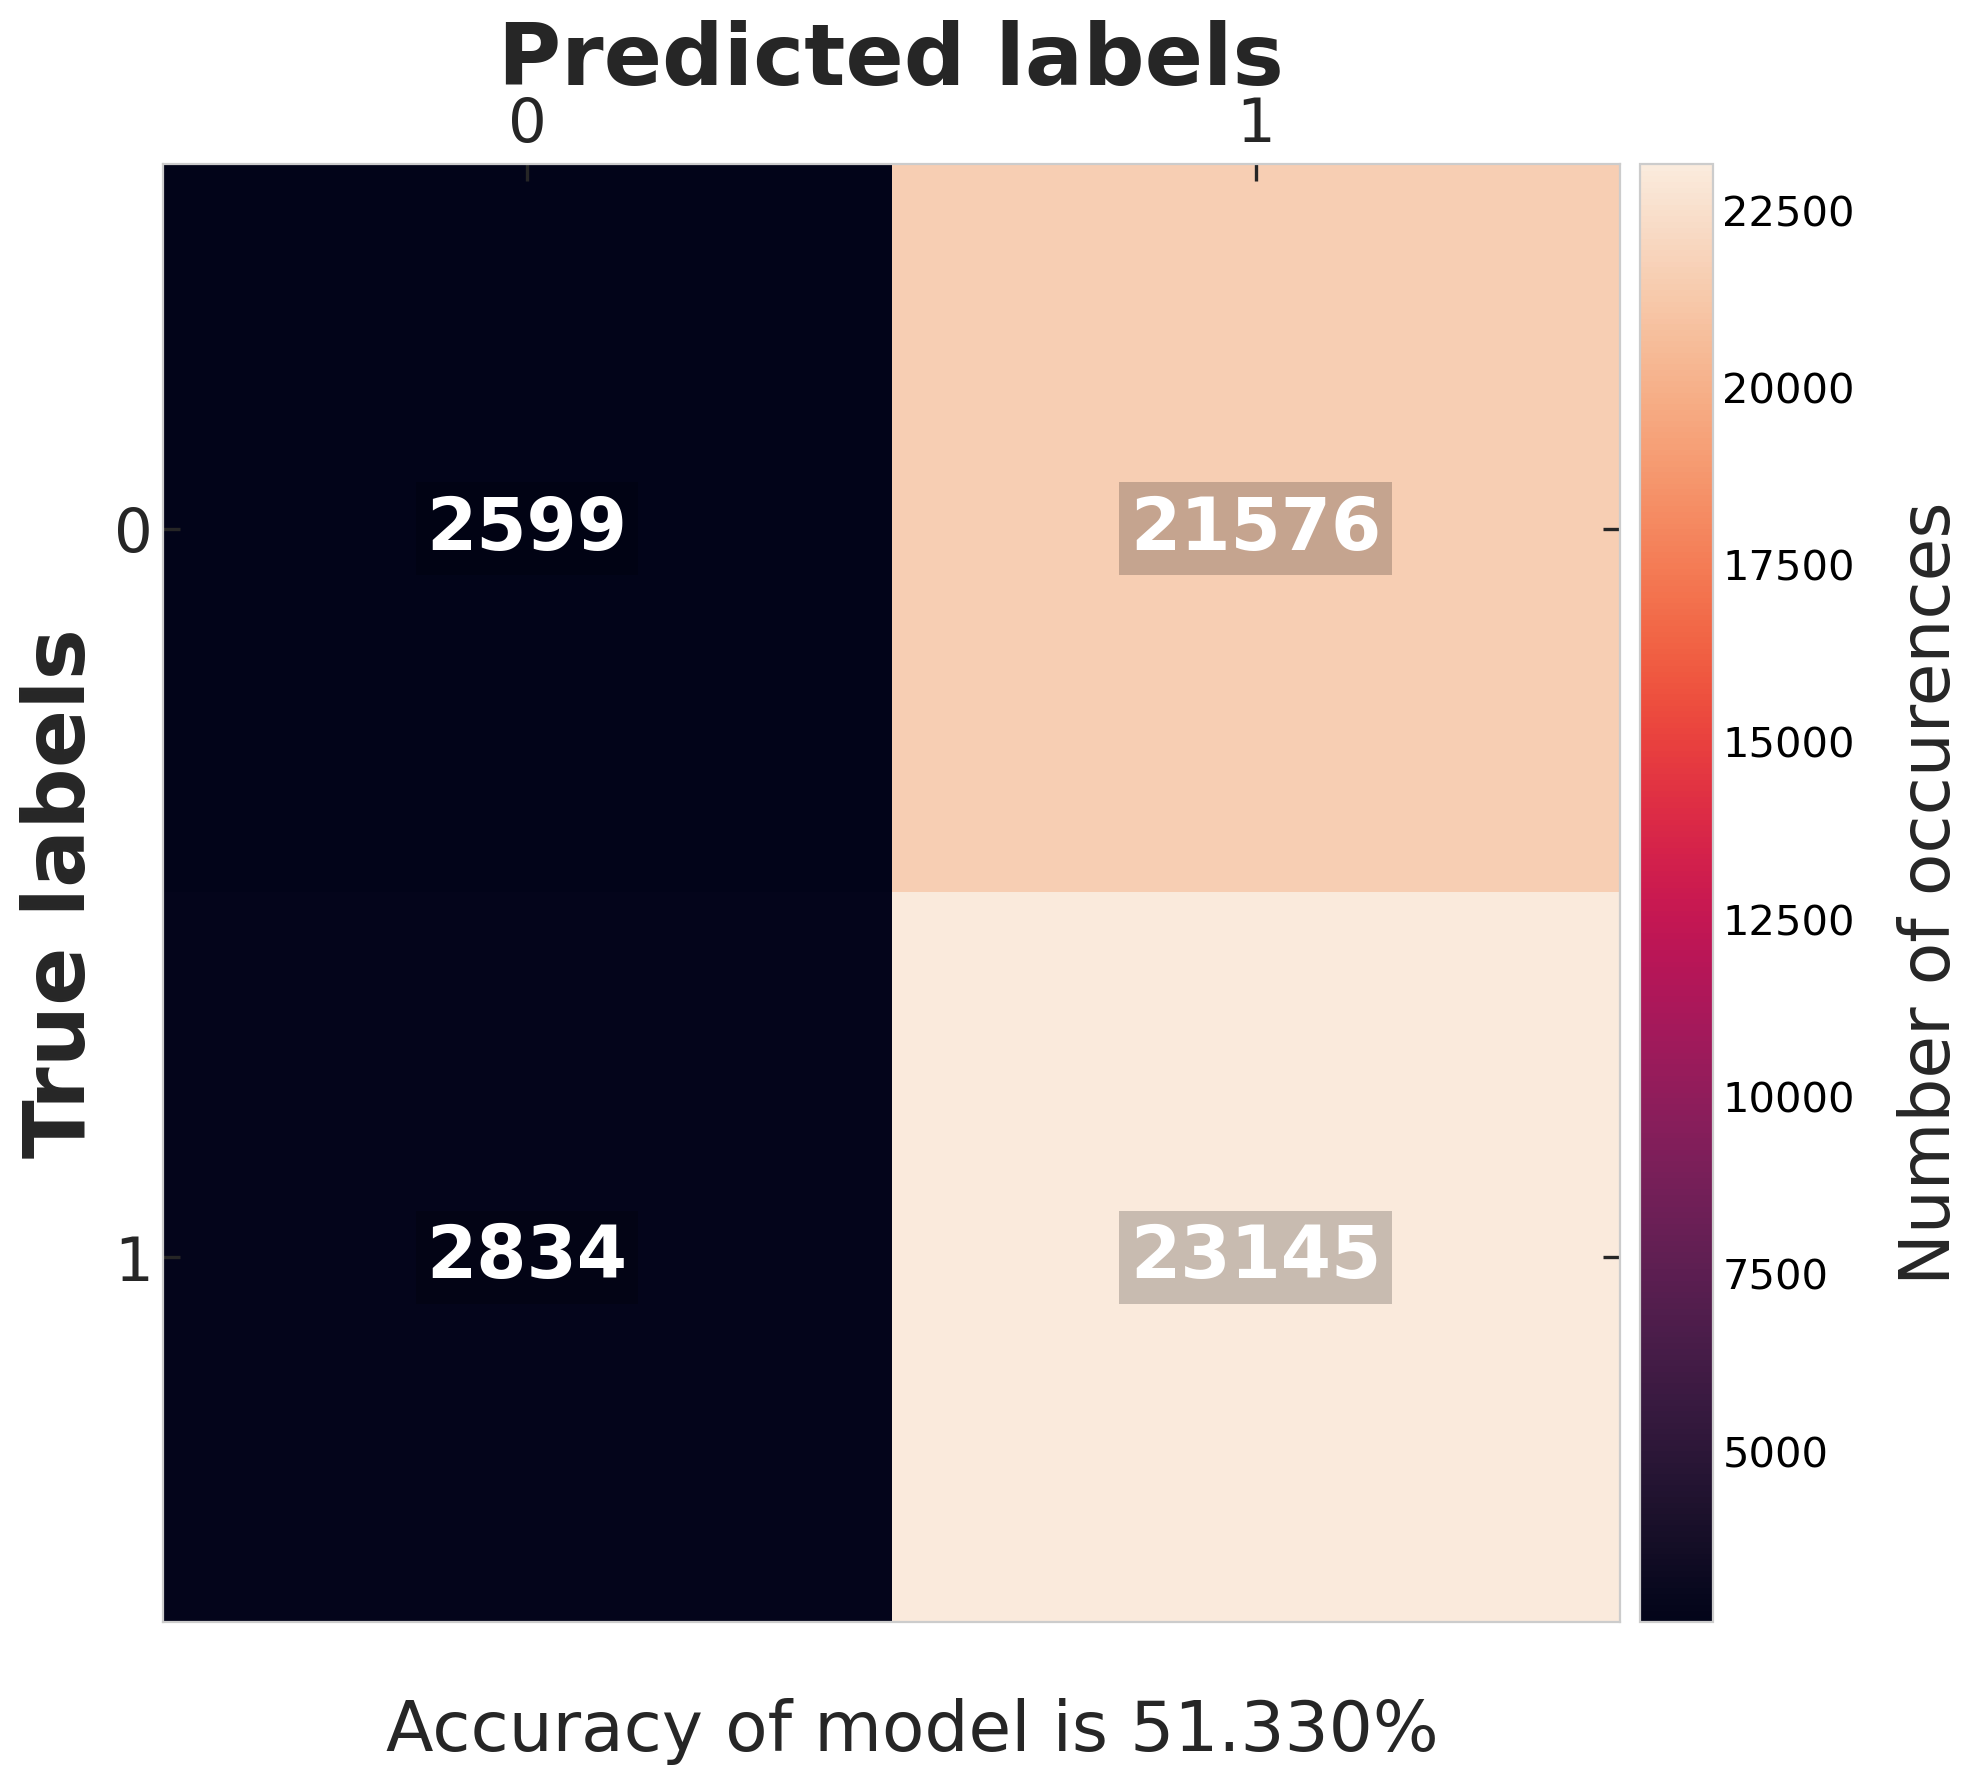
\includegraphics[width=0.99\linewidth]{./images/fig_12_ridge_abtest.png} 
			\caption{Predicting \texttt{abtest}}
		\end{subfigure}
		\begin{subfigure}{0.32\textwidth}
			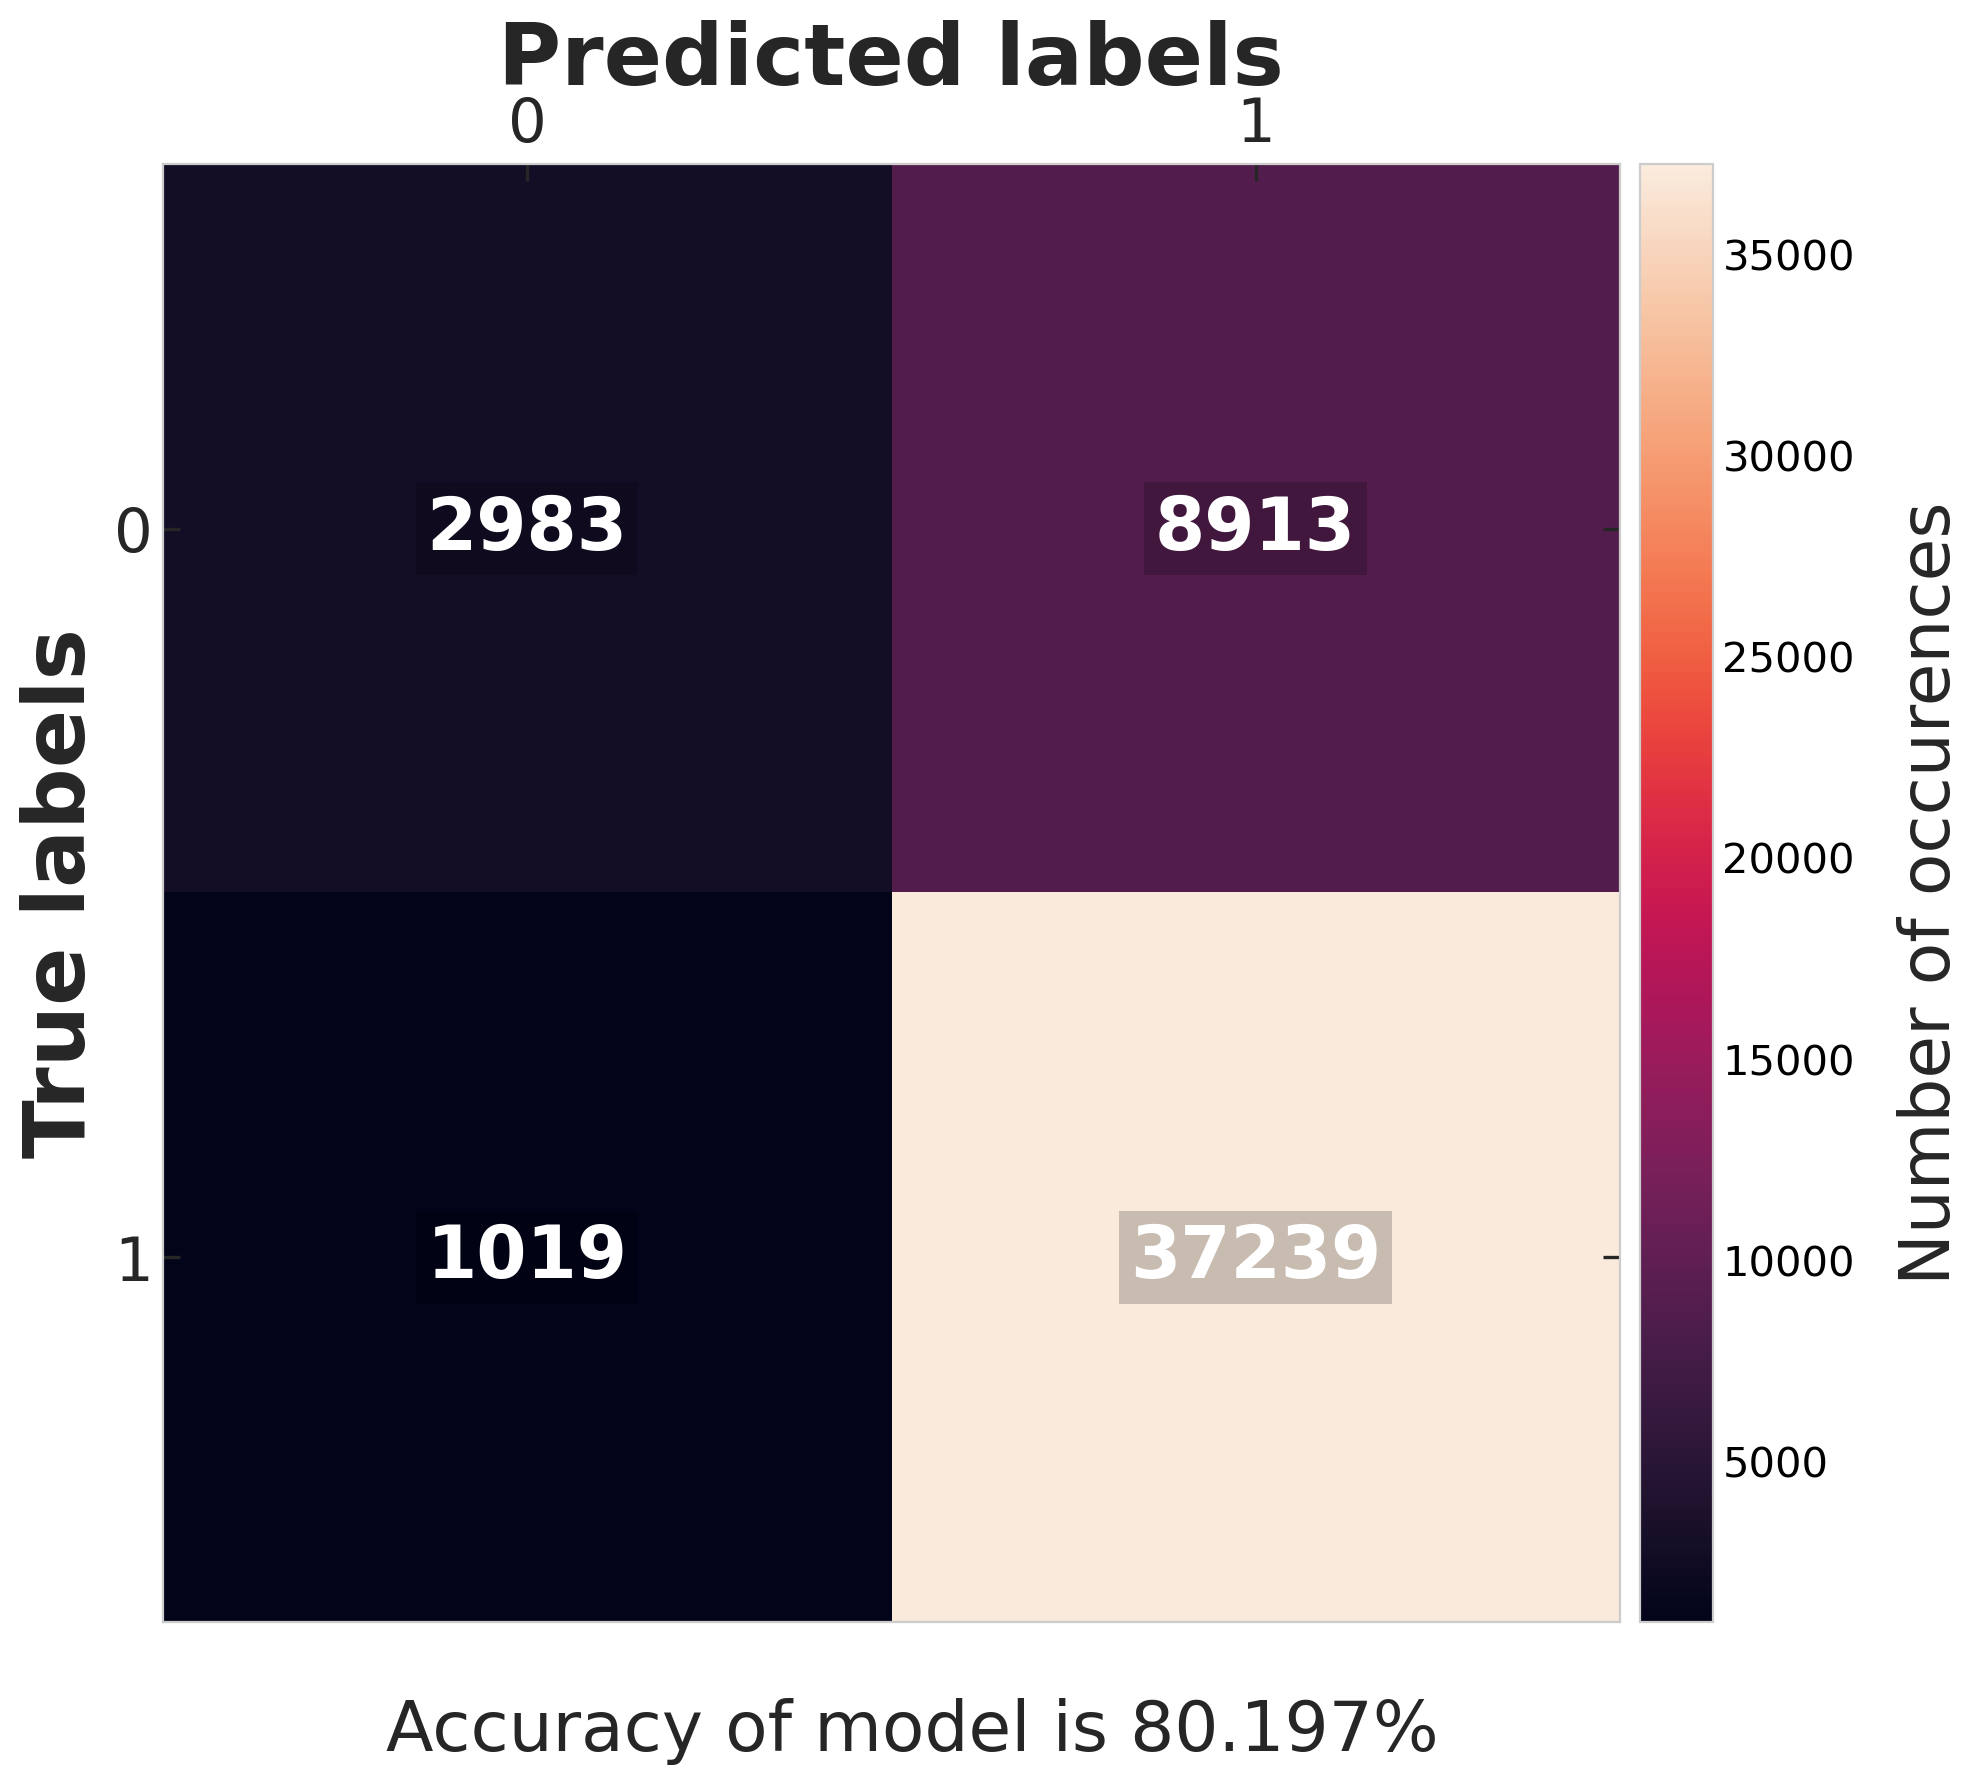
\includegraphics[width=0.99\linewidth]{./images/fig_13_ridge_gearbox.png} 
			\caption{Predicting \texttt{gearbox}}
		\end{subfigure}
		\begin{subfigure}{0.32\textwidth}
			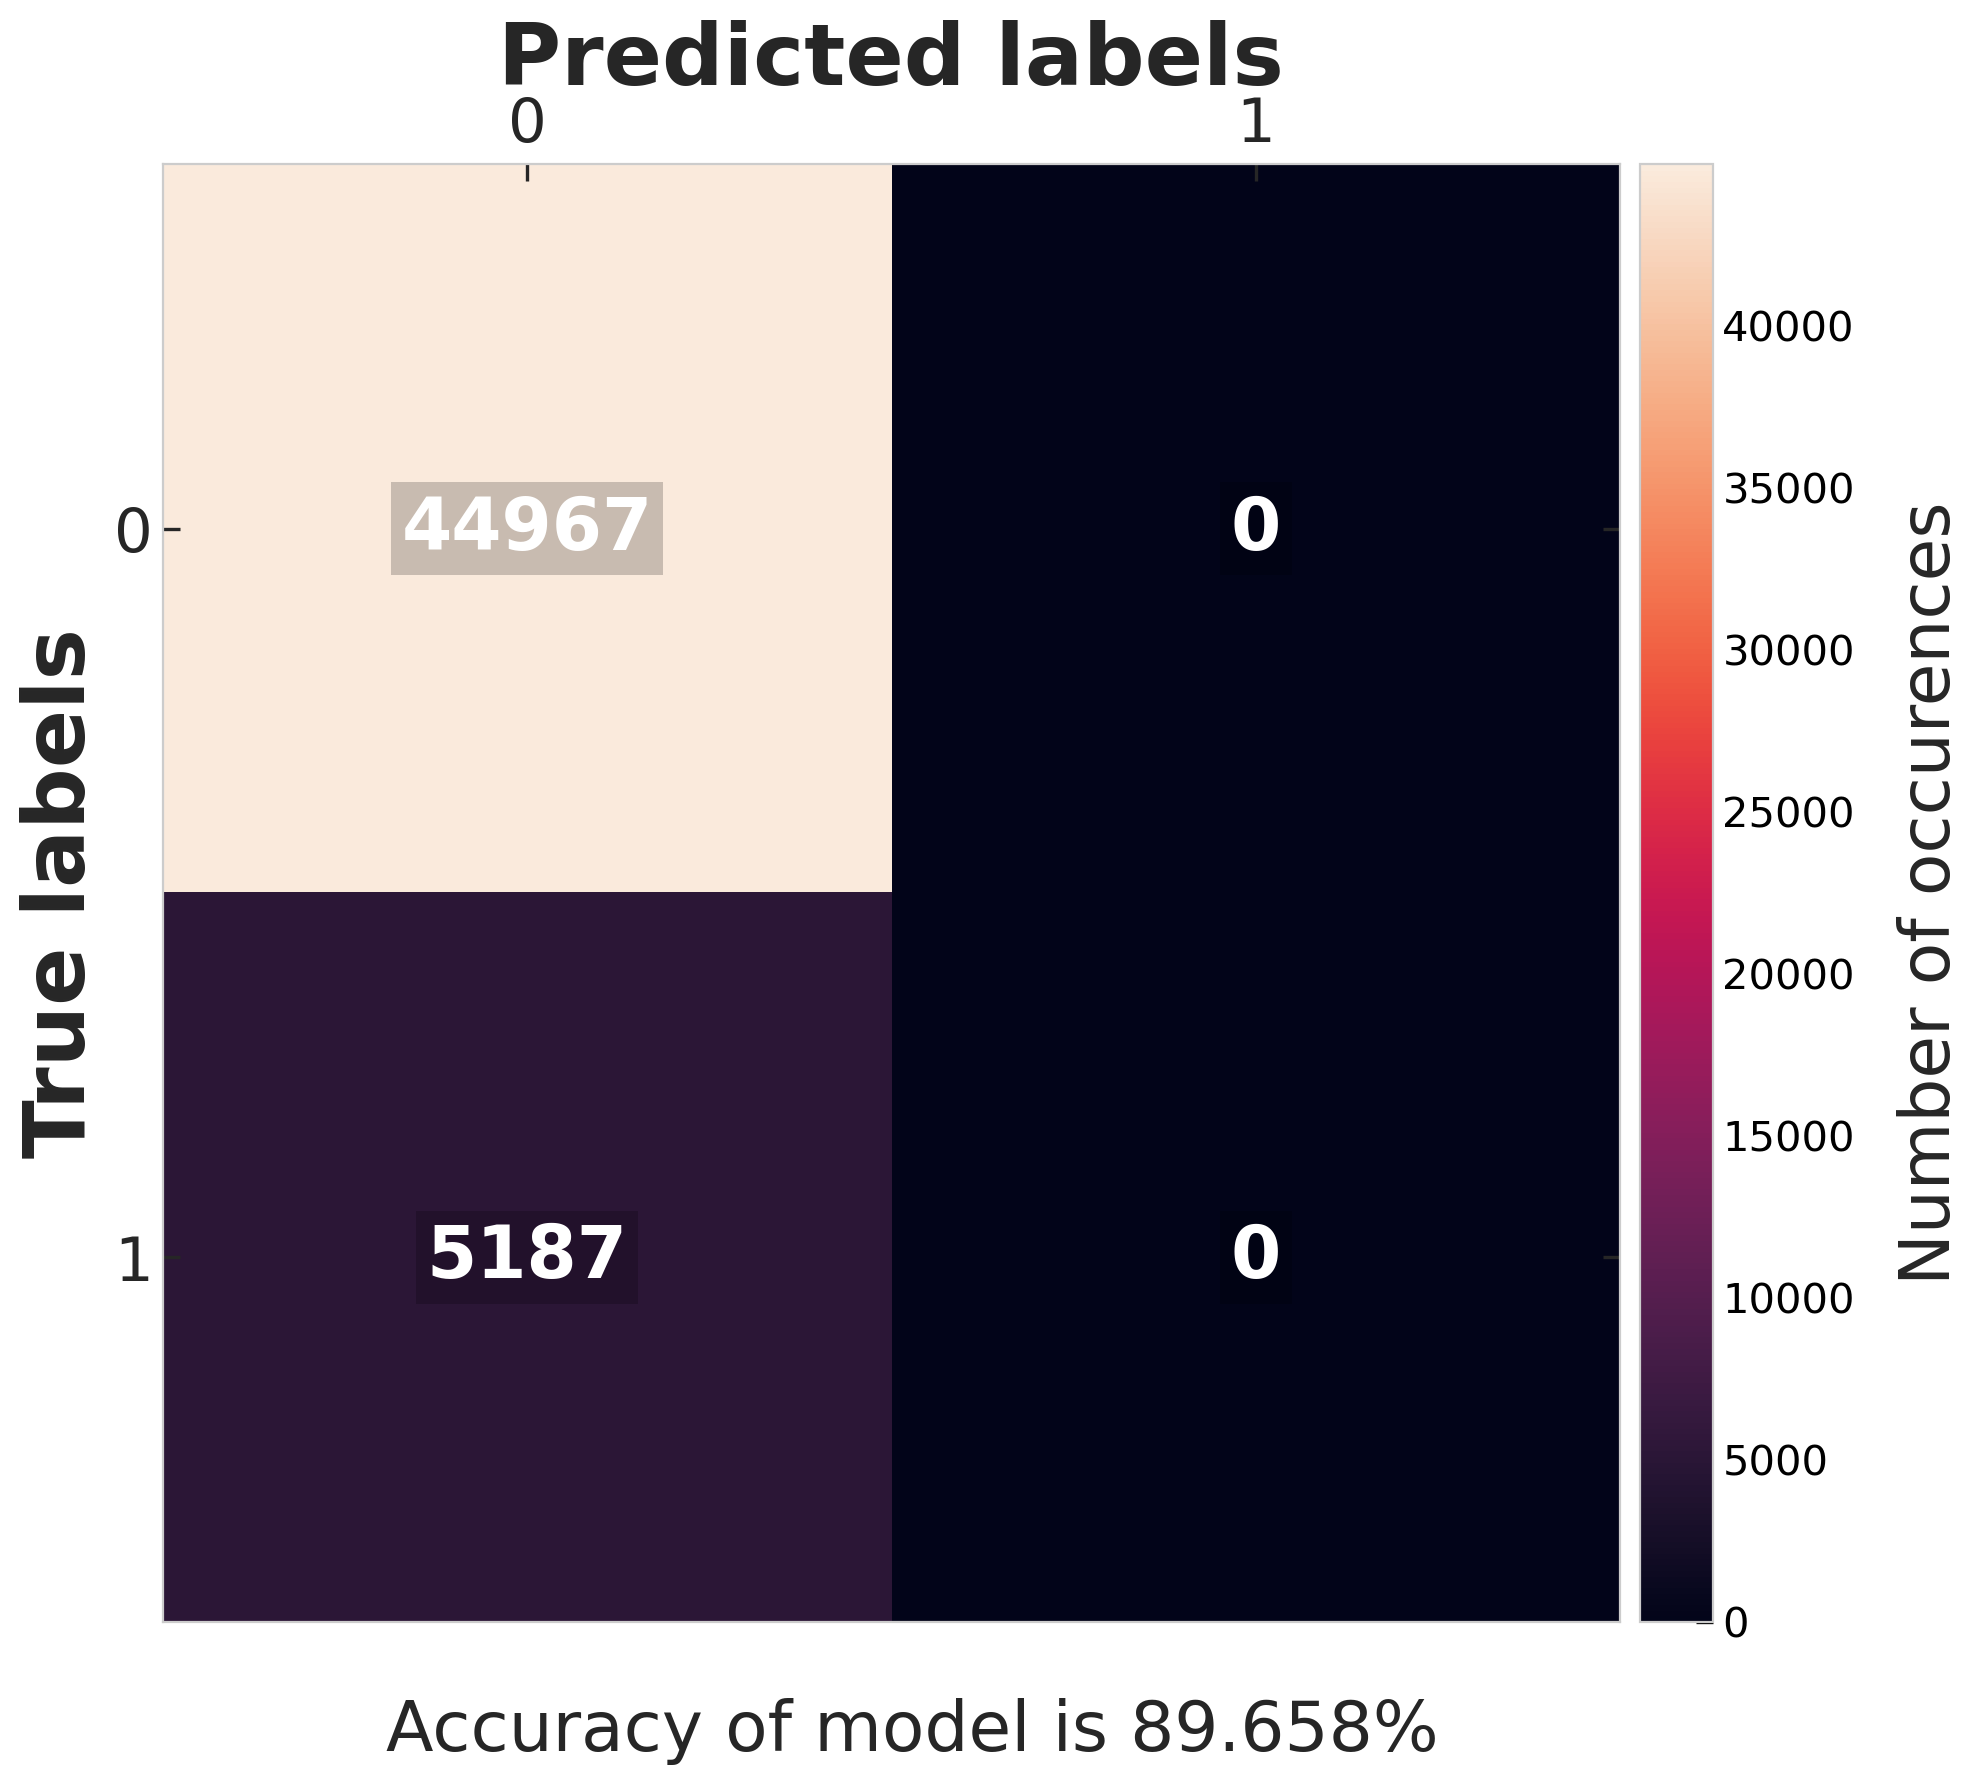
\includegraphics[width=0.99\linewidth]{./images/fig_14_ridge_notrepaired.png} 
			\caption{Predicting \texttt{notRepairedDamage}}
		\end{subfigure}
		\captionof{figure}{Training a ridge classifier on the continuous variables to predict binary labels in the dataset. Here the effect of overfitting is much more obvious and qualifies the ridge classifier method basically unusable.}
	\end{center}
\end{figure}

\subsection{Predicting price and brand of cars}
Predicting the \texttt{brand} and \texttt{price} features are probably the most interesting questions speaking in terms of this dataset. This is certainly possible, but not quite trivial in case of the given data. The features \texttt{price}, \texttt{gearbox} and \texttt{powerPS} features would very likely be able to tackle this problem. After several attempts however I failed to find any meaningful way to implement the binary gearbox variable into the model. The \texttt{powerPS} features supported by the \texttt{soldMin} feature does not helped at all neither. My results can be seen on Fig. 11., Fig. 12. and Fig. 13.

\subsection{Implement a Bayesian model with \texttt{pyro.ai} or \texttt{TF Probability}}
Maybe next time. I've played with the idea, because a Bayesian model would be probably very useful here working with a number of categorical/categorizable features. Creating a simple Bayesian graph would be probably the best here to explore the CPT between these features and predict eg. the binned \texttt{price} feature given all other conditions. The hard part itself lies in the creation of the graph and I have zero idea which nodes should I connect with each other, not even speaking about the direction of edges. Addressing this problem a structure learning algorithm should be implemented, but than that would be a much longer project work...
\newpage
\section{Discussion}
As seen on my results, I've mostly failed miserably compared to the usual outcomes of my homeworks. I've showed, that the gearbox variable maybe can be predicted reliably with a simple linear regression, but basically nothing else.
\newpage
\section{Figures for price prediction}
\begin{figure}[h]
	\begin{center}
		\begin{subfigure}{\textwidth}
			\centering
			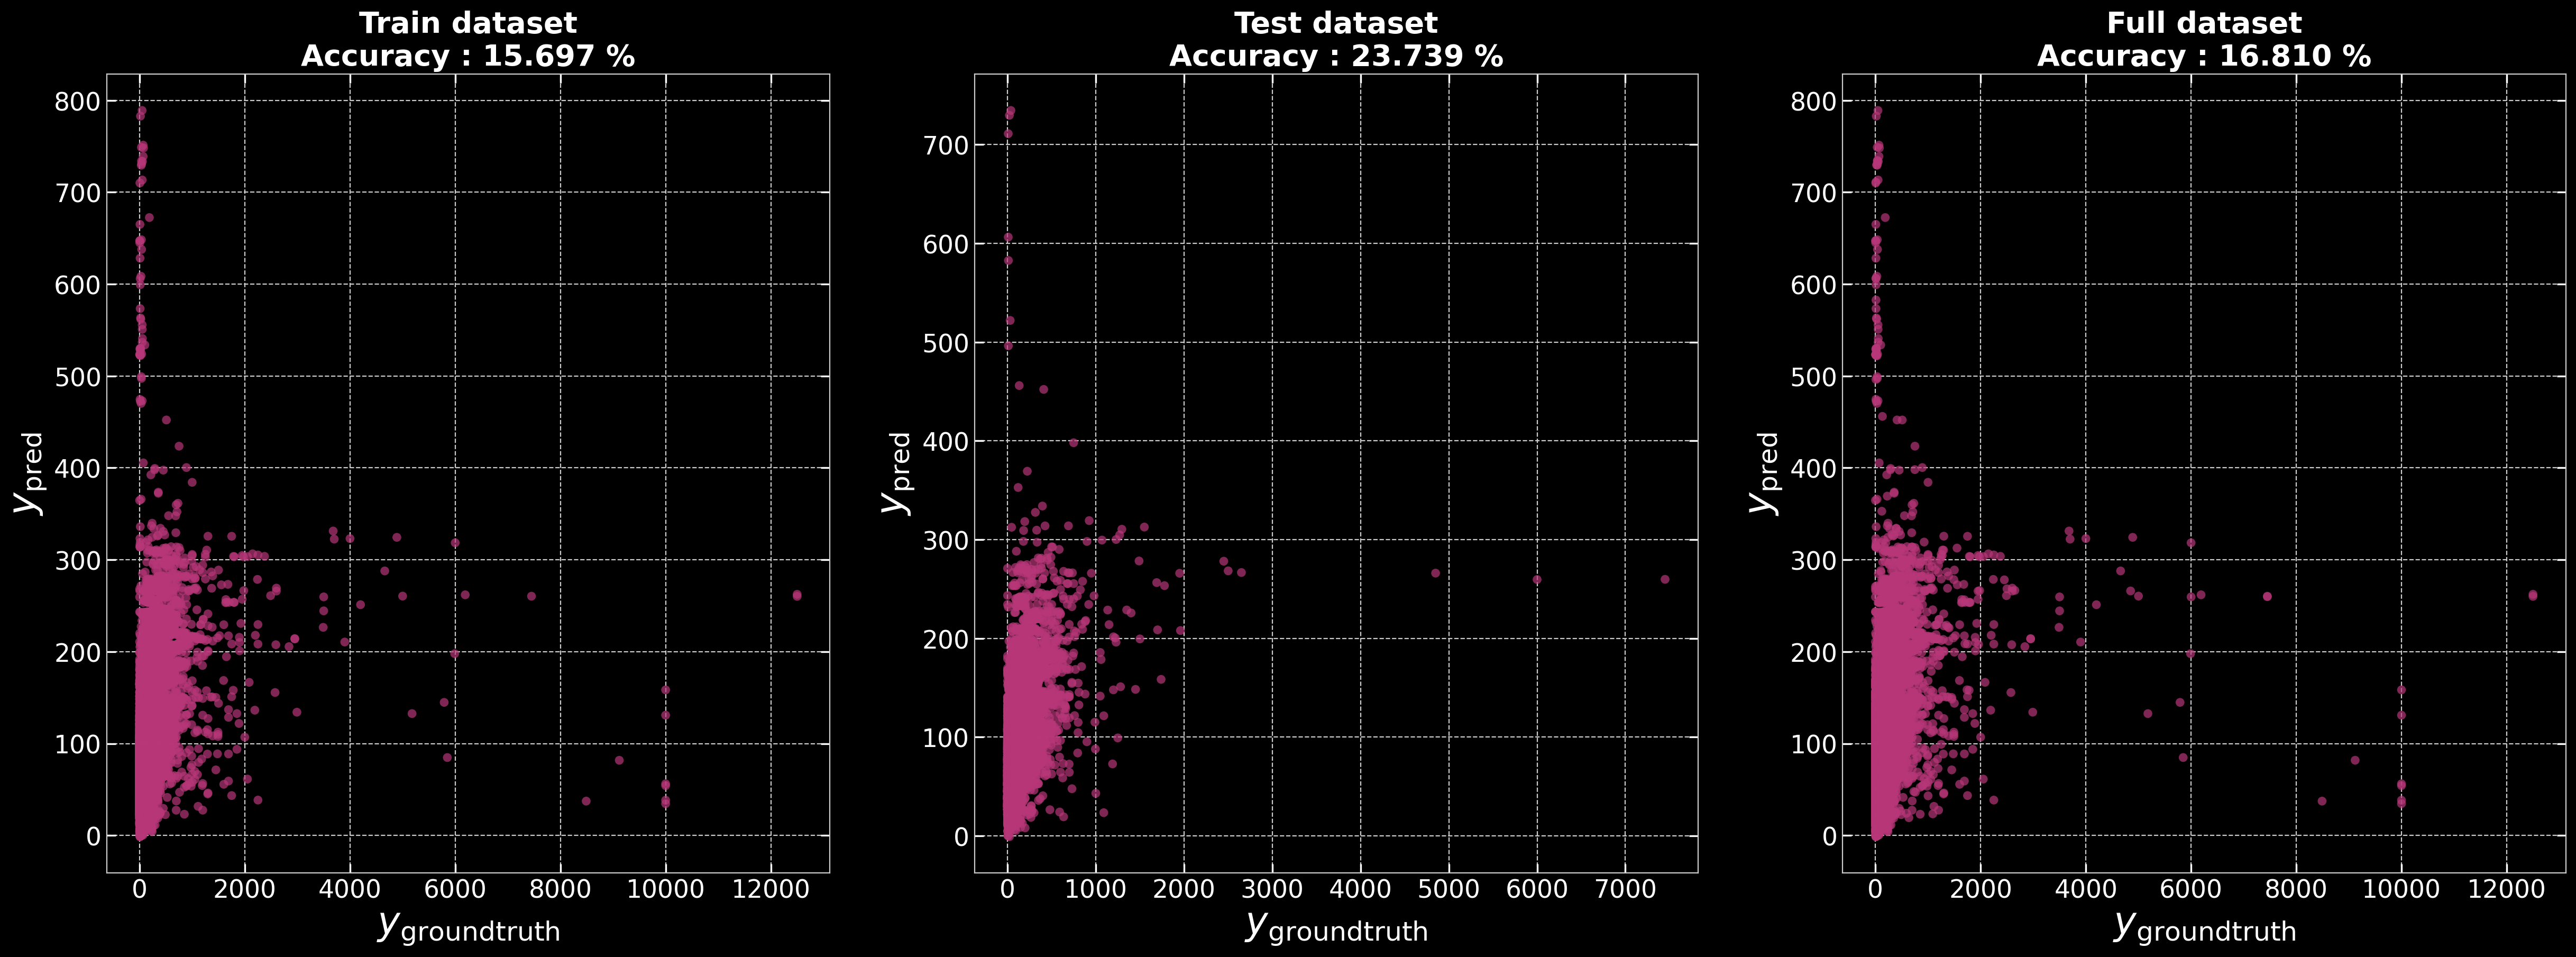
\includegraphics[width=0.9\linewidth]{./images/fig_15_ealstic_price.png}
			\caption{ElasticNet model}
		\end{subfigure}
		\begin{subfigure}{\textwidth}
			\centering
			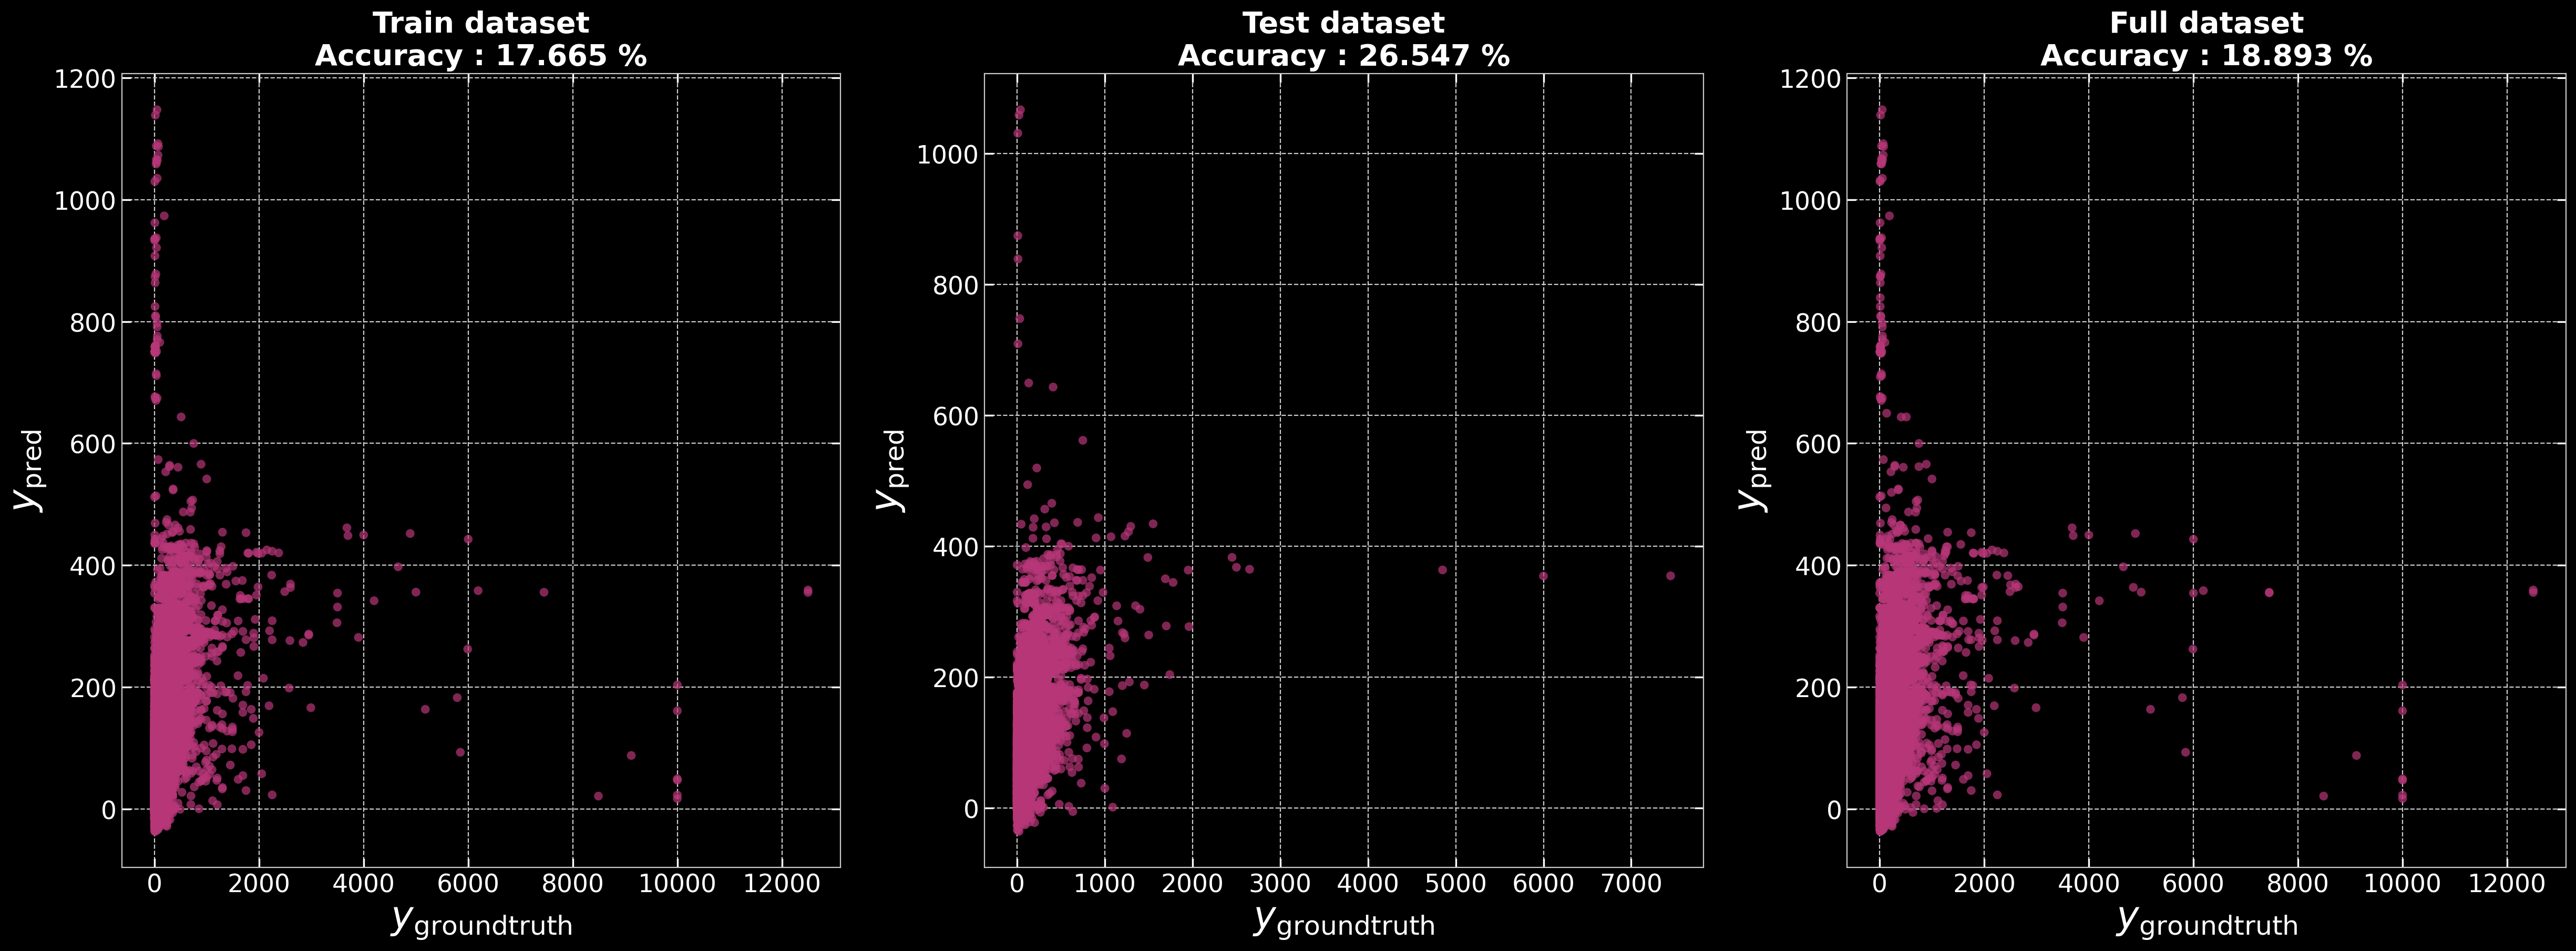
\includegraphics[width=0.9\linewidth]{./images/fig_16_linear_price.png}
			\caption{Linear regression model}
		\end{subfigure}
		\begin{subfigure}{\textwidth}
			\centering
			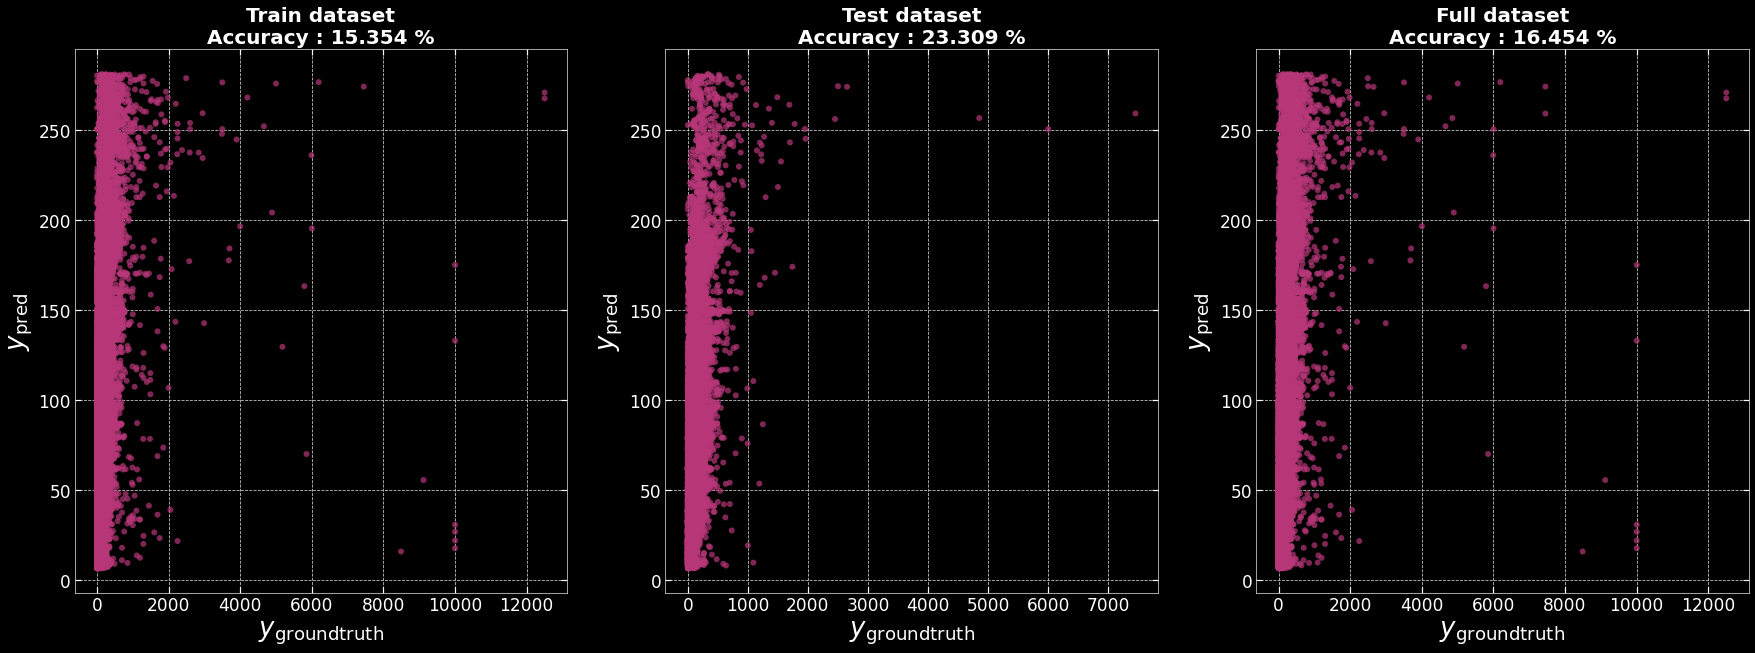
\includegraphics[width=0.9\linewidth]{./images/fig_17_svm.png} 
			\caption{SVM regression model}
		\end{subfigure}
		\captionof{figure}{Predicting the \texttt{price} with different models using the features \texttt{gearbox}, \texttt{powerPS} and \texttt{soldMin}.}
	\end{center}
\end{figure}